\documentclass[12pt]{article}

\usepackage{sbc-template}
\usepackage[utf8]{inputenc}
\usepackage{graphicx,url}
\usepackage[brazil]{babel}   
\usepackage[usestackEOL]{stackengine}
\usepackage[latin1]{inputenc}  
\usepackage{scalefnt}
\usepackage{float}

\usepackage{amssymb}
\usepackage{amsmath}
\usepackage{graphicx}

\sloppy

\title{Estrutura conceitual do Modelo para Agentes Normativos}

\begin{document} 

\section{Objetivo}

Um dos interesses deste estudo reside na investigação, dentro do contexto computacional, de cenários onde os agentes cometem erros durante a execução de algum atividade. Tendo em vista esses erros, eles podem prejudicar a si mesmos como seus colegas. Assim sendo, esse estudo investiga esse cenário por meio de um modelo que incorpora normas (instruções claras que devem ser fornecidas a um agente), violação (ocorre quando um agente descumpri uma norma) e sanção (consequências decorrentes de uma violação desta norma). Não apenas isso, mas nesse cenário há a consideração de que essas questões estão atreladas aos artefatos que são usados pelos agentes. Esses artefatos são objetos passivos que estão sujeitos a influencia da ação dos agentes. Os artefatos são usados para representar objetos como ferramentas e máquinas, por exemplo. 

Os pesquisadores consideram, neste estudo, que as violações não estão relacionadas apenas aos artefatos, mas também nas relações entre todas as entidades existentes ao longo do cenário. As entidades compõem todos os elementos ativos (agentes) bem como os elementos passivos (artefatos) vinculados ao meio. Assim sendo, entidade é todo o ente que existe por si mesmo. As condições ambientais onde os agentes e os artefatos estão inseridos também são considerados neste estudo. O entendimento que se tem por condição ambiental consiste em um dado processo que existe no ambiente e que, de certa forma, pode influenciar a execução das atividades dos agentes. Como condições ambientais têm-se por exemplo os seguintes eventos; chuva, sol, vento e neve. 

Não é do interesse deste estudo investigar condições normativas cuja caráter punitivo advém de sanções administrativas e jurídicas que ocorre no que tange a decisão de uma certa autoridade. Assim sendo, o modelo resultante deve ser capaz de representar situações onde os agentes sofrem consequências físicas negativas resultantes de uma cadeia de causalidade que foi ocasionada pelo erro de alguém (usando, para isso, o conceito de norma, violação e sanção). Dada essa circunstância, a representação tratada neste estudo deve trabalhar, em sua estrutura interna, o conceito de risco. É digno de nota que o termo risco apresenta um espectro semântico bastante amplo podendo ser usado nos mais diferentes contextos possíveis (ex. risco financeiro de um dado ativo). Por conta disto, é necessário frisar que neste texto o vocábulo risco é usado no mesmo significado atribuído pela comunidade de Engenharia de Segurança. 

As relações causais, em muitos casos, são complexas demais para serem mapeadas em seu mínimos detalhes. Por conta disso, muitos estudos realizam uma tratativa probabilística dessas relações. O modelo a que se propõem esse estudo não pretende tratar nenhuma das duas linhas. Para isso, os pesquisadores decidiram por fazer uso do conceito de possibilidade. Essa situação é usada para compreender casos onde um agente sofre consequências negativas por meio de eventos que possuem uma certa natureza aleatória. O cenário neste estudo se restringe apenas aos mundos onde esses eventos ruins (apresentam consequências ruins aos profissionais envolvidos) se tornam possíveis dado ao vacilo de algum profissional em uma atividade anterior.   


Muitas atividades praticas são definidas em termos de objetivos. Não apenas isso, mas essa linha é muito bem verificada pela acadêmica científica e está presente em modelos de \textit{SMA} dos mais diversos, tal como o \textit{MOISE}. Assim sendo, a representação a que se propõem neste estudo orienta os agentes em termos de objetivos que devem ser atingidos. Um objetivo define um estado de mundo $S_g$. Assim sendo, se o mundo está um estado $S_a$ onde $S_a \neq S_g$, os agentes devem fazer o possível para que o estado do mundo seja $S_g$. Neste estudo, um estado mundo é dado por todos os estados de todas as entidades.

Não é possível definir um agente dentro de uma sociedade sem ao menos definir o seu papel (ou função). Por exemplo, se há o interesse em construir um modelo de \textit{SMA} que seja apropriado para descrever o cenário de um hospital, essa representação pode ser entendida como demasiadamente pobre se não levar em consideração a função do médico. Assim sendo, o modelo presente neste texto deve considerar o papel do agente. 

Agentes são máquinas de estado que possuem autonomia para tomar decisões. Em termos genéricos, é possível classificar dois tipos de agentes; reativos e cognitivos. Os agentes reativos apenas reagem a estímulos do meio. A outra classe de agentes são os cognitivos, possuem estados internos e tem a capacidade de realizar raciocínios. O tipo de agente (bem como sua estrutura interna no que diz respeito a tomada de decisões) não faz parte do objeto de estudo desta pesquisa. Assim sendo, o modelo em interesse não delimita o vocabulário para estruturar a concepção do agente propriamente dito. 


Neste estudo, os pesquisadores têm interesse em apresentar um vocabulário específico no que tange aos conceitos presentes nesta seção. Esse modelo, portanto, deve ser capaz de representar organizações tais como trabalhadores em uma obra, industrias, profissionais no âmbito hospitalar e estruturas deste gênero entendendo como se dá as violações em âmbitos específicos (falta de ferramentas, não conseguir executar procedimentos apropriados, executar uma atividade cujo momento não era adequado para isso). 

A fim de se obter uma estrutura representacional formal com aspecto de especificidade altamente notório, este estudo faz uso da teoria dos modelos (onde os conceitos são escritos em termos de conjuntos) e lógica de predicados (usado para definir as relações entre os conceitos). Não apenas isso, há o interesse em definir regras que tem como por finalidade exprimir a transição de estados possessível de mundo. Assim sendo, essas regras, neste modelo, são definidas em termos de relações de implicabilidade que são delineadas pelas \textit{Cláusulas de Horn}.


Para o propósito aqui posto, se não há infinitas maneiras, há ao menos um numero muito variado de formas para construir um modelo com os objetivos aqui definidos. Contudo, esse texto desbrava ao menos uma das formas de se realizar isso, analisa a abordagem sobre um estudo e define uma comparação com os modelos já existentes dada pela comunidade acadêmica. A análise comparativa é estruturada em termos de; conceitos (verificar quais são similares e quais são diferentes), relações entre os conceitos, capacidade de generalização (quanto mais mundos possíveis o modelo é capaz de descrever, mais genérico o é), capacidade de especificação tendo como referência circunstâncias que correspondem ao presente neste texto introdutório e uma verificação sobre como esses critérios se dão dos modelos em relação a um dado estudo de caso aqui presente. 


\section{Exemplo - Estudo de Caso}

Sete profissionais de linha viva (profissionais que realizam manutenção em equipamentos elétricos energizados) são designados com o propósito de realizar a substituição de um isolador de pedestal. Os papeis desses desses profissionais são; 1 supervisor, 5 executores. A manutenção deve ser executada apenas sobre as seguintes condições: céu ensolarado e umidade relativa do ar menor que 70 porcento. Todos os profissionais devem possuir os EPI's necessários: capacete, óculos de sol, roupa isolante e antichamas, luvas isolantes e botas isolantes. Os profissionais que entram no potencial devem estar vestidos de roupa condutiva e cabo guarda. As ferramentas necessárias para resolver esse problema são: bastão garra de diâmetro 64 x 3600 mm, sela de diâmetro 65 , colar, corda de fibra sintética, carretilha, chave com catraca, bastão universal, soquete adequado, locador de pino e bastão com soquete multiangular. O método selecionado para esse tipo de manutenção é a distância onde o eletricista não acessa diretamente o potencial, mas faz isso por intermédio de um bastão isolante. A substituição do isolador de pedestal pode ser escrita nos seguintes objetivos: 


\begin{enumerate}
	\item Limpar, secar e testar corda.
	\item Instalar Bastão Garra na estrutura com o pedestal a ser substituído.
	\item Instalar sela com colar na estrutura
	\item Amarrar o bastão na parte superior da estrutura com a corda.
	\item Amarrar o olhal do bastão ao cavalo da sela atrás de uma corda.
	\item Instalar um segundo conjunto bastão e sela no lado oposto da estrutura.
	\item Enforcar um estropo de Náilon no corpo do isolador.
	\item Colocar a extremidade do estropo no gancho da corda de serviço.
	\item Afrouxar os parafusos do conector que prendem a barra ao isolador.
	\item Terminar de retirar os parafusos com o bastão com o soquete multiangular.
	\item Elevar a barra através da corda que une a sela ao bastão.
	\item Apertar o colar através da porca borboleta.
	\item Segurar firmemente a corda de serviço.
	\item Sacar parafusos da base da coluna.
	\item Baixar o isolador ao solo
	\item Içar o Isolador
	\item Colocar Parafusos na base da coluna.
	\item Baixar a barra para que a mesma apoie no novo isolador.
	\item Colocar os parafusos do conector que prende a barra ao novo isolador. 
	\item Retirar Equipamentos
\end{enumerate}

\section{Modelo}

O modelo deste estudo é uma linguagem definida em $\Omega_{model}$, onde;
\begin{eqnarray}
\Omega_{model} = \{\Omega_{class},\Omega_{relation},\Omega_{rule}\}
\end{eqnarray}

O conjunto $\Omega_{class}$ é o conjunto que representa os conceitos usados para descrever o domínio de interesse deste modelo. O conjunto $\Omega_{relation}$ contem conjuntos cartesianos de relacionamento $R \subset \{(a,b)|a\in A \wedge b \in B\}$. Esses conjuntos representam as relações entre os conceitos $\Omega_{class}$. Neste texto faz-se o uso da notação $r(a,b)$ em vez de usar da notação $r = (a,b)$. O conjunto $\Omega_{rule}$ contem relações de implicabilidade $x \to y$ que representam as regras do modelo. 


\subsection{Definição - $\Omega_{class}$}

	Cada item da lista a seguir corresponde a um subconjunto de $\Omega_{class}$.

\begin{enumerate}
	\item $Entity = \{e_1, ..., e_n\}$ - conjunto de todas as Entidades.  
	\item $Agent = \{ag_1, ..., ag_n\}$ - conjunto dos Agentes.
	\item $Artefact = \{at_1, ..., at_n\}$ - conjunto dos Artefatos.
	\item $EntityGoal = eg = \{e_n,...,e_m\}$ - conjunto das Entidades que devem estar presentes para concluir um determinado objetivo $g_i$.
	\item $Relation = \{r_1, ..., r_n\}$ - conjunto dos Relacionamentos entre as entidades.	
	\item $RelationGoal = rg =\{r_n, ..., r_m\}$ - conjunto dos Relacionamentos que devem estar presentes para concluir um determinado objetivo $g_i$.		
	\item $Role = \{\rho_1, ..., \rho_n\}$ - conjunto dos Papeis que um determinado agente pode exercer no grupo onde é um participante.	
	\item $Goal = \{g_1, ..., g_n\}$ - conjunto dos Objetivos que devem ser alcançados pelos demais agentes.
	\item $Condition = \{c_1, ..., c_n\}$ - conjunto das Condições que devem ser mantidas ao longo da execução dos objetivos (ex. o dia deve está ensolarado para que a manutenção ocorra).
	\item $ConditionGoal = cg = \{c_n, ..., c_m\}$ - conjunto de condições que devem ser mantidas para concluir um determinado objetivo $g_i$.
	\item $Risk = \{risk_1, ..., risk_n\}$ - conjunto dos Riscos na ocorrência de Eventos Ruins.
	\item $Possibility = \{false,true\}$ - conjunto das possibilidades de Eventos Ruins. 
	\item $Fatality = \{f_1, ..., f_n\}$ - conjunto das fatalidades que acontecem na existência de um evento ruim. 	
	\item $agg = \{ag_n,...,ag_m\}$ - agentes que atingiram um determinado objetivo. 
	\item $ago = \{ag_n,...,ag_m\}$ - agentes que atingiram um determinado objetivo e eram obrigados a isso. 
\end{enumerate}

A lista a seguir apresenta as relações clássicas definidas pela teoria dos conjuntos, cujas quais são; $\cap,\equiv,\subset,\cup$ 

\begin{enumerate}
	\item $Entity \equiv Agent \cup Artefact$
	\item $Agent \cap Artefact = \emptyset $.
	\item $ agg \subset Agent$
	\item $ ago \subset Agent$ 
	\item $\{agg_1,...,agg_n\} \subset Agent$	
	\item $ GoalPrerequisite \subset Goal$
	\item $ ConditionGoal \subset Condition$
	\item $ EntityGoal \subset Entity$		
	\item $ RelationGoal \subset Relation$
\end{enumerate}


\subsection{Definição dos Predicados - $\Omega_{relation}$}

Os subconjuntos de $\Omega_{relation}$ são dados pelos itens da lista a seguir;

\begin{enumerate}
	\item $relationHas(r_l,e_i,e_k)$ onde $i \neq j$ - Um relacionamento $r_l$ é composto por uma entidade $e_i$ e $e_k$ onde $e_i$ não pode ser igual a $e_j$.	
	\item $hasRole(ag_n,\rho_m)$ - Um agente $ag_n$ tem um papel $\rho_m$.
	\item $hasObligation(\rho_m,g_j)$ - Quem assume o papel $\rho_m$ é obrigado a concluir o objetivo $g_j$.
	\item $hasPermission(\rho_m,g_j)$ - Quem assume o papel $\rho_m$ tem a permissão de concluir o objetivo $g_j$.
	\item $isReached(g_k)$ - O objetivo $g_k$ foi alcançado.
	\item $stopIn(g_n,agg_m)$ - Para pelo menos um dos agentes que constituem o conjunto $agg_m$ o objetivo $g_n$ foi encerrado. 	 				
	\item $stopIn(g_n)$ - A atividade como um todo teve de ser finalizada em $g_n$.	 			
	\item $nextGoal(g_i,g_j)$ - Quando o objetivo $g_i$ é alcançado, o agente deve ir para o próximo objetivo $g_j$. 	
	\item $hasCondition(g_i,cg_n)$ - Um objetivo do tipo $g_i$ possui certas condições $c$ que deve estar presentes e devem se manter durante toda execução deste objetivo. Essas condições $c$ devem estar contidas em $cg_n$. 
	\item $hasEntity(g_i,eg_m)$ - Um objetivo $g_i$ tem um conjunto de entidades $eg_m$ onde todas as entidades presentes neste conjunto devem estar presentes no momento da execução desse objetivo.
	\item $hasRelation(g_i,rg_n)$ - Um objetivo $g_i$ tem um conjunto de relacionamentos $rg_n$ onde todos esses relacionamentos devem ser feito para que este objetivo seja concluído.
	\item $isPresent(X), X = cg_n,c_k,rg_k,r_k,eg_k,e_k$ - Define se $X$ está presente no instante em análise, sendo que $X$ pode ser $cg_n,c_k,rg_k,r_k,eg_k,e_k$.
	\item $tryReach(ag_i,g_j)$ - Um determinado agente $ag_i$ tenta alcançar o objetivo $g_j$. Para o agente tentar alcançar um dado objetivo, o papel dele ao menos deve ter permissão para isso.  
	\item $violationCondition(ag_i,g_j,c_k)$ - Um determinado agente $ag_i$ comete uma violação de condição no objetivo $g_j$ sobre a condição $c_k$. 
	\item $violationRelation(ag_i,g_j,r_k)$ - O agente $ag_i$ comete uma violação de Relacionamento no objetivo $g_j$ por não realizar o relacionamento $r_k$. 
	\item $violationEntity(ag_i,g_j,e_k)$ - O agente $ag_i$ comete uma violação de Entidade no objetivo $g_j$ por tentar alcançar esse objetivo sem ter a entidade $e_k$ presente.  	
	\item $hasRisk(X,risk_j,f_m), X = c_k,r_k$ - $X$ está associada a um risco $risk_k$ com uma certa fatalidade $f_m$. Esse $X$ pode ser uma condição $c_k$ ou um relacionamento $r_k$. 
	\item $consequenceOfBadEvent(g_k,ag_i,risk_j,f_m)$ - Agente $ag$ sofre as consequências do risco $risk_j$ com a fatalidade $f_m$
	\item $hasPossibility(r_l,p_m)$ - Possibilidade $p_m$ do evento $r_l$ gerar alguma consequência ruim, mesmo que os profissionais desenvolvam a atividade com perfeição sobre o ponto de vista técnico e de segurança. A possibilidade $p_m$ pode assumir apenas dois valores; $true,false$, ou seja - ou essa possibilidade existe ou não existe. 	
	\item $affects(r_k,r_n)$ - Se uma relação $r_k$ não for feita, ou se essa relação for mal feita, então ela afeta negativamente alguma outra relação $r_n$ com a possibilidade de algo errado inicialmente dado por $false$ ser mudado para $true$. 	
	\item $happensBadEvent(r_m)$ - Acontece o evento ruim em uma dada relação $r_m$.		
	\item $lastGoal(g_i,\rho_m)$ - é o ultimo objetivo $g_i$ associado a um certo papel $\rho_m$.		
\end{enumerate}

\subsection{Definição das Regras - $\Omega_{rule}$}

Cada relação de implicabilidade a seguir é uma regra do modelo que faz parte do conjunto $\Omega_{rule}$. 

\begin{equation}\label{rel1}
	hasObligation(\rho_m,g_j) \to hasPermission(\rho_m,g_j)  
\end{equation}

\begin{eqnarray}\label{rel3}\nonumber
	hasCondition(g_i,cg_n) \wedge \neg isPresent(c_k) \wedge (c_k \in cg_n) \wedge tryReach(ag_m,g_i) \to \nonumber \\  
	violationCondition(ag_m,g_j,c_k) 
\end{eqnarray}

\begin{eqnarray}\label{rel4}\nonumber
	hasRelation(g_i,rg_n)\wedge \neg isPresent(r_k) \wedge (r_k \in rg_n) \wedge tryReach(ag_m,g_i) \to \nonumber \\
	violationRelation(ag_m,g_i,r_k)
\end{eqnarray}

\begin{eqnarray}\label{rel5}\nonumber
	hasEntity(g_i,eg_n) \wedge \neg isPresent(e_k) 	\wedge (e_k \in eg_n) \wedge tryReach(ag_m,g_i) \to \nonumber \\ violationEntity(ag_m,g_i,e_k)  
\end{eqnarray}

\begin{eqnarray}\label{rel9}\nonumber
	violationCondition(ag_m,g_i,c_k)  \wedge hasRisk(c_k,risk_j,f_m) \to \\ 
	consequenceOfBadEvent(g_i,ag_m,risk_j,f_m)
\end{eqnarray}

\begin{eqnarray}\label{rel10}\nonumber
	violationRelation(ag_m,g_i,r_k) \wedge hasRisk(r_k,risk_j,f_m) \to \\ 
	consequenceOfBadEvent(g_i,ag_m,risk_j,f_m)
\end{eqnarray}

\begin{eqnarray}\label{rel11}\nonumber
	violationRelation(ag_m,g_i,r_k) \wedge affects(r_k,r_n) \wedge hasPossibility(r_n,false) \to \\  
	hasPossibility(r_n,true)
\end{eqnarray}

\begin{eqnarray}\label{rel12}
	violationEntity(ag_m,g_i,e_k) \to stopIn(g_i)
\end{eqnarray}


\begin{eqnarray}\label{rel13}\nonumber
	hasPossibility(r_k,true) \wedge  happensBadEvent(r_k) \wedge hasRelation(g_i,rg_n) \wedge (r_k \subset rg_n) \nonumber \\ 
	\wedge hasRisk(r_k,risk_j,f_m) \wedge tryReach(ag_m,g_i) \nonumber \\ 
	\to consequenceOfBadEvent(g_i,ag_m,risk_j,f_m) \nonumber \\
\end{eqnarray}

\begin{eqnarray}\label{rel14}
	consequenceOfBadEvent(g_k,ag_m,risk_j,f_m) \to stopIn(g_k)
\end{eqnarray}

\begin{eqnarray}\label{rel15}
	\neg stopIn(g_k,agg_n) \wedge (ago_n \subset agg_n) \to isReached(g_k)
\end{eqnarray}

\begin{eqnarray}\label{rel16}
	hasRole(ag_n,\rho_m) \wedge hasPermission(\rho_m,g_j) \wedge nextGoal(g_i,g_j) \wedge isReached(g_i) \nonumber \\
	\to tryReach(ag_n,g_j) \nonumber \\
\end{eqnarray}

\begin{eqnarray}\label{rel16}
	hasRole(ag_n,\rho_m) \wedge hasPermission(\rho_m,g_i) \wedge lastGoal(g_i,\rho_m) \wedge isReached(g_i) \nonumber \\
	\to stopIn(g_i) \nonumber \\
\end{eqnarray}


\subsection{Definindo Conceitos de Norma, Violação e de Sanção}

Sistemas multiagentes normativas não podem ser descritos sem considerar três conceitos importantes; norma, violação e sanção. 

\begin{enumerate}
	\item \textbf{Norma}: Usado para determinar o comportamento dos agentes.
	\item \textbf{Violação}: Ocorre quando o agente não cumpre com uma norma.
	\item \textbf{Sanção}: Consequências punitivas que acontecem ao agente dada a ocorrência de uma violação.	
\end{enumerate}

Essas definições são usadas em diversos estudos na área de sistemas multiagentes \cite{dastaniNormativeMultiAgentProgram}, \cite{multiagentsystem}, \cite{amodelmultiagentsystemdynamicrelationship} e \cite{ontologynormative}. Nesse estudo, a violação é tratada nos predicados $violationCondition(ag_i,g_j,c_k)$, $violationRelation(ag_i,g_j,r_k)$ e $violationEntity(ag_i,g_j,e_k)$. Usando a mesma sistemática de regras adotada em \cite{dastaniNormativeMultiAgentProgram}, as relações \ref{rel3}, \ref{rel4},\ref{rel5} define as condições necessárias para que uma violação venha a acontecer. Ainda dentro da abordagem apresentada em \cite{dastaniNormativeMultiAgentProgram}, as relações \ref{rel9}, \ref{rel10} são sanções. Isso, pois definem consequências negativas aos agentes tendo em vista a ocorrência da violação. 


\subsection{Justificando a Existência das Regras}


\subsubsection{Regra \ref{rel1}}

Se uma gente é obrigado a fazer algo, então esse agente deve ter a permissão para isso. Caso contrário, por um impedimento sistemico, um agente nunca conseguirá cumprir com aquilo a que ele é obrigado a fazer. Essa é a finalidade da regra \ref{rel1}, onde uma obrigação implica necessariamente em uma permissão. Outros modelos adotam uma abordagem similar a essa \cite{mosieframework}. 

\subsubsection{Regra \ref{rel3}}

Representar condições que devem ser mantidas ao longo de toda a execução da atividade bem como as consequências de praticar uma determinada atividade dado a ausência de pelo menos uma das condições é um aspecto sobre o qual este modelo se propõem a representar. Para definir a ocorrência da violação se faz necessário saber quais são as condições vinculadas ao objetivo. Caso contrário não é possível identificar quais condições devem ser mantidas ao longo da tentativa de se alcançar um objetivo. Por consequência, não é possível realizar qualquer afirmação feita sobre essas condições. A consideração dessas relações acontece por meio predicado $hasCondition(g_i,cg_n)$. 

Outro aspecto relevante consiste saber se a condição necessária está presente na tentativa do agente alcançar um dado objetivo. Assim sendo, é necessário a presença do predicado $isPresent(c_k)$. O negado de $isPresent(c_k)$ define que uma dada condição $c_k$ não está presente. Ainda sim, $hasCondition(g_i,cg_n)$, $isPresent(c_k)$ não são suficientes, pois $cg_n$ é um conjunto e $c_k$ é um elemento que pode ou não pertencer ao conjunto $cg_n$. Portanto, é necessário considerar se $c_k$ pertence a $cg_n$ e isso é feito através de $c_k \in cg_n$. 

Os predicados considerados até o momento são necessários, porém não são suficientes. Isso, pois apenas com eles não é possível definir qual é a situação do agente em relação ao objetivo. Por exemplo, é possível considerar um cenário onde pelo menos uma das condições necessárias para atingir o objetivo não está presente. Contudo, não é razoável, considerando o conceito de violação de condição empregado neste estudo, afirmar que o agente cometeu uma violação de condição sobre esse cenário sendo que não há informação sobre a situação da tentativa do agente alcançar o objetivo. Assim sendo, se o agente tentar alcançar o objetivo mesmo com pelo menos uma condição inexistente, então esse agente cometeu uma violação de condição, contudo se o agente não tentou alcançar o objetivo em análise então ele não cometeu violação alguma. Então, a informação no que diz respeito ao gente deve ser considerada nessa relação de implicabilidade e isso acontece por meio do predicado $tryReach(ag_m,g_i)$.

 
\subsubsection{Regra \ref{rel4}}
Para levar em consideração violações sobre se o agente sabe ou não manipular algum tipo de relação, se faz necessário buscar por relações de implicabilidade que verificam as seguintes circunstâncias: relações que devem ser feitas para que um determinado objetivo possa ser atingido $hasRelation(g_i,rg)$, se a relação em análise é uma relação que pertence a todas as relações necessárias para findar esse objetivo $r_k \in rg_g$, verificar se a relação em análise está presente quando o agente realiza a atividade $isPresent(r_k)$ e levar em consideração o ato do agente tentar executar a atividade $tryReach(ag_m,g_i)$. A violação acontece quando, na reunião de todas essas circunstâncias, uma das relações não se faz presente $\neg isPresent(r_k)$. Para essa situação, $violagionRelation(ag_m,g_i,r_k)$ tem que ser verdadeiro. 

Considerando que uma violação de relacionamento acontece quando um agente tenta alcançar um objetivo sem realizar um ou mais dos relacionamentos necessários para que esse objetivo seja satisfeito com sucesso, é possível avaliar a necessidade das circunstâncias presentes na relação de implicabilidade deste modelo por analisar o que acontece na ausência de cada uma delas. Seguindo por essa linha, supondo uma situação onde não se verifica as relações relevantes para um objetivo, logo não é possível dizer se a ausência de uma violação em específico é relevante para o objetivo em análise. Assim sendo, não é possível afirmar quando acontece uma determinada violação. 

Supondo uma situação onde não se verifica as relações que foram concluídas durante o ato da manutenção. Neste cenário é possível saber quais relações são necessárias para alcançar um determinado objetivo, mas deste conjunto não é possível definir qual dessas relações foram alcançadas. Se não se sabe afirmar qual das relações um agente conseguiu realizar, não se sabe qual dessas relações um agente deixou de fazer. Não sabendo esta ultima, não se sabe se ocorreu uma violação dessa relação. Assim sendo, só é possível afirmar algo sobre a ocorrência de uma violação de relação se for possível analisar se as relações necessárias para um dado objetivo foram ou não cumpridas. 

Supondo uma situação onde não se verificar se um agente tentou realizar o objetivo. Nesta situação não é possível analisar quem cometeu a violação. Além disso não é possível considerar se a presença ou a ausência das relações são relevantes ou não para alcançar o objetivo, pois não se pode localizar a ocorrência dessas relações nos momentos onde elas devem acontecer (que é quando o agente tenta alcançar o objetivo dessas relações). 

\subsubsection{Regra \ref{rel5}}

Para verificar violações onde um agente tenta executar um determinado procedimento sem ter todas entidades (ex. ferramentas, colegas) requisitadas, é necessário construir uma expressão de implicabilidade que considera quais são as entidades importantes para a execução do objetivo $hasEntity(g_i,eg_n)$, considere quais as entidades que estão presentes no ambiente durante o ato da execução $isPresent(e_k)$,$e \in eg_n$ e que considere se um agente tentou alcançar o objetivo $tryReach(ag_m,g_i,e_k)$.

Se uma violação de entidade é definida como sendo a tentativa de um agente alcançar um determinado objetivo sem ter todas as entidades para isso, então é possível verificar a necessidade de todas as circunstâncias por analisar o que acontece na ausência delas. Supondo não ser possível verificar quais entidades são necessárias para alcançar um determinado objetivo. Então não é possível afirmar quais entidades devem estar presentes durante a tentativa do agente em alcançar um determinado objetivo. Por consequência, também não é possível identificar quais entidades estão ausentes logo, neste caso não é possível fazer qualquer afirmação sobre presença ou ausência sobre violação por ausência de uma entidade. 

Supondo não ser possível afirmar sobre a presença de uma entidade necessária para conclusão de um determinado objetivo. Assim sendo, também não é possível realizar qualquer afirmação sobre uma violação deste gênero. 

Suponto não ser possível definir se um agente tentou ou não alcançar um dado objetivo. Então também não é possível saber se a entidade estava presente no momento em que deve estar presente. Como consequência disto, não é possível fazer nenhuma afirmação sobre essa violação.


\subsubsection{Regras \ref{rel9} e \ref{rel10}}

O propósito da relação \ref{rel9} consiste representar uma sanção sobre ocorrência de uma violação de condição. Uma violação dessa natureza pode gerar consequências decorrentes do risco pelo qual o profissional estava sendo submetido. Isso envolve situações como; queimaduras,lesões,fraturas e morte. Esse modelo considera essas consequências como sanção por violar uma determinada norma. Assim sendo, uma relação de implicabilidade que tem como por comprometimento representar uma sanção desta natureza deve considerar os riscos, fatalidade e o elemento causador desta situação. Decorrente disso, o predicado $hasRisk(c_k,risk_j,f_m)$ representa as relações entre a condição faltante, a natureza do risco e o grau de fatalidade associado. O predicado $consequenceOfBadEvent(g_i,ag_m,risk_j,f_m)$ define que o evento ruim realmente aconteceu sobre esse agente. 


A relação \ref{rel10} se enquadra na mesma natureza. Contudo, em vez de considerar uma violação de condição, a relação \ref{rel10} considera violações do tipo de relacionamento. Essa relação é necessária pois visa representar as consequências negativas de não se fazer um relacionamento necessário para a manutenção. 


\subsubsection{Regra \ref{rel11}}


Uma das finalidades deste modelo consiste representar o seguinte cenário: agente A comete um erro, contudo as consequências ocorrem apenas um tempo depois sobre o agente B. Esse modelo considerou a violação de relacionamento como causa deste tipo de situação pois no caso em estudo foi possível identificar certas relações que se não forem feitas não geram consequenciais de imediato para os profissionais envolvidos no meio, contudo alguém pode sair prejudicado em etapas futuras da atividade.

Por exemplo, um ambiente hipotético onde um eletricista deve medir a condutividade de um bastão universal é uma situação que pode exemplificar a aplicação desta relação. Se o eletricista não realizar a relação entre a entidade condutímetro com a entidade bastão universal, nenhum profissional sai prejudicado de imediato. Contudo, se o bastão estiver com isolamento comprometido, o agente que for manipular a ferramenta poderá ser submetido a uma corrente elétrica elevadíssima gerando morte do indivíduo.

Essa situação pode ser tratada por considerar uma possibilidade $p$ sobre uma dada relação $r_n$. Se $p$ é $false$, então a ocorrência de um evento ruim só se torna realidade se o agente cometer alguma ação que resulte nisso. Contudo, se $p$ é $true$, então existe a possibilidade de ocorrer um evento ruim vinculado a $r_n$ mesmo que o agente execute o relacionamento com a mais alta maestria.

Para representar esse tipo de situação que se faz necessário a existência da regra \ref{rel11}. Neste caso, como a situação é decorrente de uma violação de relacionamento, se faz necessário usar o predicado $violationRelation(ag_m,g_i,r_k)$. Além disso, é necessário considerar quais relacionamentos são afetados por $r_k$ por isso a necessidade do predicado $affects(r_k,r_n,p)$. Por último, se faz necessário avaliar um predicado que vincula o relacionamento afetado $r_n$ com a possibilidade $p$, sendo isso feito por $hasPossibility(r_n,p)$.


\subsubsection{Regra \ref{rel12}}

Como a conclusão de um determinado objetivo acontece em função de certas entidades, a ocorrência da uma violação de entidade resulta, necessariamente, em uma impossibilidade de alcançar o objetivo em análise. Logo, a manutenção como um todo fica inviabilizada de ser concluída. É possível considerar um cenário onde os agentes adaptam outras entidades para sanar a entidade faltante. Contudo, o modelo proposto neste texto não trata esse tipo de situação com a finalidade de evitar maiores complexidades. Para uma relação de implicabilidade que tem como por finalidade representar esse tipo de situação, deve necessariamente considerar a ocorrência da violação $violationEntity(ag_m,g_i,e_k)$ e representar o encerramento da atividade, representado pelo predicado $stopIn(g_i)$.

\subsubsection{Regra \ref{rel13}}

Dada a ocorrência de uma violação de relacionamento que resulte na regra \ref{rel11}, um dado relacionamento  $r_n$ passa a ter uma possibilidade da ocorrência de um evento ruim mesmo que o agente execute $r_n$ com a mais alta maestria tanto sobre a perspectiva técnica como sobre a perspectiva de segurança. Assim sendo, a regra \ref{rel13} tem a finalidade de representar as situações onde, sobre essa possibilidade, um evento ruim $happensBadEvent(g_n,r_n,ag_k)$ se torna verdade. 

Como o evento ruim consiste nos riscos vinculados ao relacionamento $r_n$, deve estar contido na regra necessariamente o predicado $hasRisk(r_n,risk_j,f_m)$, caso contrário não tem como saber qual risco, qual fatalidade afeta o agente $ag_k$. Dentro desta perspectiva, também é necessário saber se o agente estava tentando executar o objetivo onde o relacionamento deve ser levado em consideração ao executar o procedimento de manutenção. Além disso, é necessário saber se o agente estava tentando alcançar o objetivo no instante que o evento ruim acontece, isso é feito por meio do predicado $tryReach(ag_m,g_i)$. O predicado $consequenceOfBadEvent(g_i,ag_m,risk_j,f_m)$ demonstra que o evento realmente aconteceu e afetou o agente de certa forma com certa intensidade.

\subsubsection{Regra \ref{rel14}}

Na ocorrência de um acidente sério os agentes não continuam a trabalhar. Assim sendo, é necessário considerar uma relação de implicabilidade onde a ocorrência de um evento ruim gera interrupção das atividades profissionais. 

\subsubsection{Regra \ref{rel15}}

O modelo deve considerar a condição de quando objetivo é definitivamente alcançado, caso contrário os agentes não serão capaz de cumprir com os próximos objetivos para os quais foram designados. Para construir esse critério é necessário considerar se não houve interrupção para todos os agentes que tentaram alcançar o objetivo. Isso é feito por meio do predicado $\neg stopIn(g_k,agg_n)$. Não só isso como é necessário considerar se todos os agentes que são obrigados a alcançar o objetivo realmente tentaram fazer isso. Assim sendo, é necessário considerar se $ago_n$ está contido em $agg_n$.   

\subsection{Diagramas que Representam o Modelo}

A figura dada por \ref{uml} apresenta a estrutura do modelo em formato de diagrama de classes.

\begin{figure}[H]
  \centering
  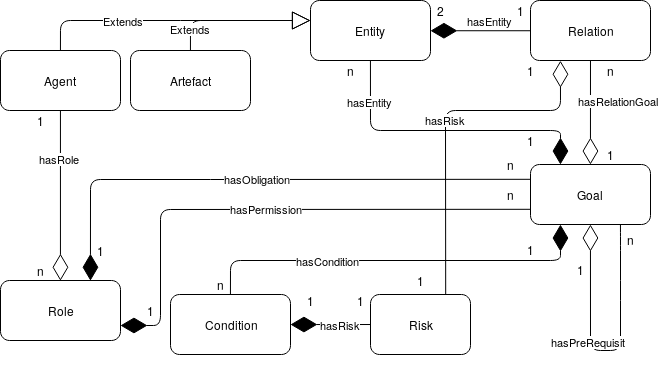
\includegraphics[width=1\linewidth]{uml20} 
  \caption{}
  \label{uml}
\end{figure}

A figura \ref{state} apresenta um diagrama de estados do modelo. 

\begin{figure}[H]
  \centering
  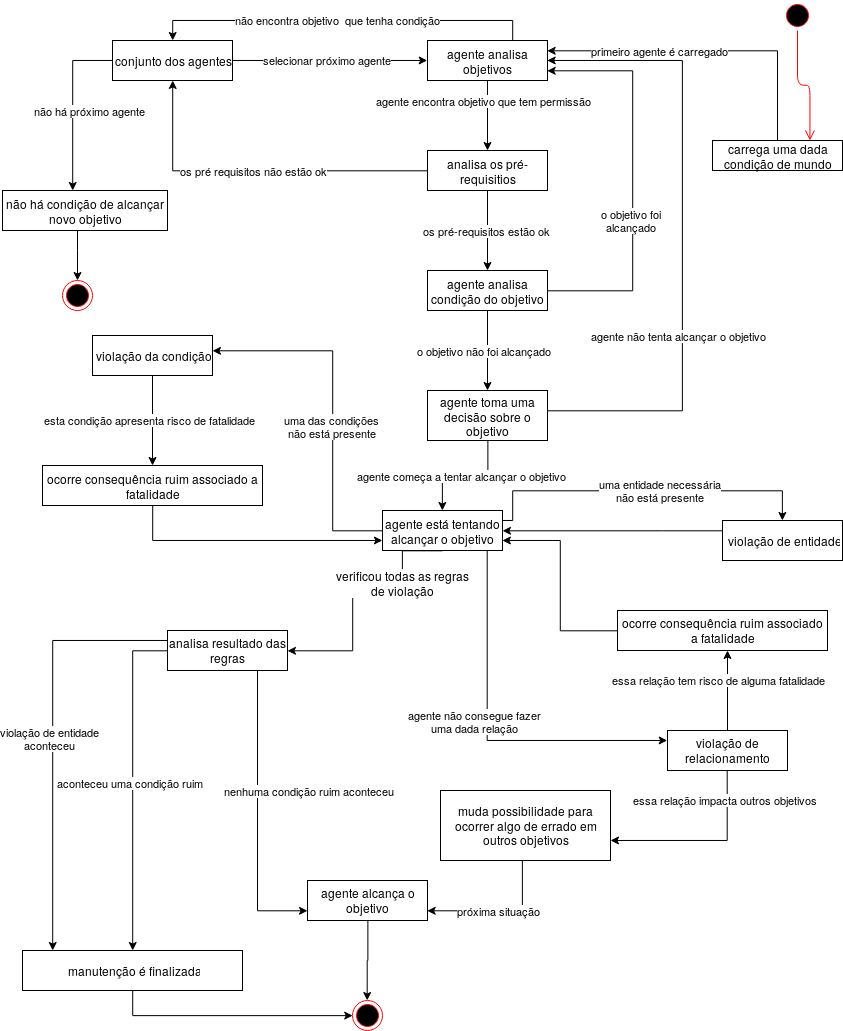
\includegraphics[width=0.9\linewidth]{DiagramaDeEstados} 
  \caption{}
  \label{state}
\end{figure}

\subsection{Modelando}

Essa subseção tem como por finalidade especificar o estudo de caso em interesse dentro da estrutura deste modelo. 

A tabela \ref{agents} apresenta todos os agentes que fazem parte da manutenção. A tabela \ref{roles} apresenta todas as funções que deverão ser exercidas pelos agentes. A tabela \ref{agentsroles} define a relação $hasRole(ag_n,\rho_m)$ onde $ag_n$ é representado pela coluna agente e $\rho_m$ é representado pela coluna papel.

\begin{table}[H]
\scalefont{0.8}
\centering
\begin{tabular}{|l|l|}
\hline
\textbf{símbolo} & \textbf{significado} \\ \hline
agente1 & Um dos agentes participantes da manutenção \\ \hline
agente2 & Um dos agentes participantes da manutenção \\ \hline
agente3 & Um dos agentes participantes da manutenção \\ \hline
agente4 & Um dos agentes participantes da manutenção \\ \hline
agente5 & Um dos agentes participantes da manutenção \\ \hline
agente6 & Um dos agentes participantes da manutenção \\ \hline
agente7 & Um dos agentes participantes da manutenção \\ \hline
\end{tabular}
\caption{Os agentes que constituem uma manutenção}
\label{agents}
\end{table}


\begin{table}[H]
\scalefont{0.8}
\centering
\begin{tabular}{|l|l|}
\hline
\textbf{papel} & \textbf{descrição} \\ \hline
supervisor & Atribui papel a outros profissionais \\ \hline
executor1 & Tem como por finalidade executar certas atividades manuais vinculadas a manutenção \\ \hline
executor2 & Tem como por finalidade executar certas atividades manuais vinculadas a manutenção \\ \hline
executor3 & Tem como por finalidade executar certas atividades manuais vinculadas a manutenção \\ \hline
executor4 & Tem como por finalidade executar certas atividades manuais vinculadas a manutenção \\ \hline
executor5 & Tem como por finalidade executar certas atividades manuais vinculadas a manutenção \\ \hline
\end{tabular}
\caption{Os papeis relevantes para a ocorrência da manutenção}
\label{roles}
\end{table}


\begin{table}[H]
\scalefont{0.8}
\centering
\begin{tabular}{|l|l|}
\hline
\textbf{agente} & \textbf{papel} \\ \hline
agente1 & supervisor \\ \hline
agente2 & executor1 \\ \hline
agente3 & executor1 \\ \hline
agente4 & executor2 \\ \hline
agente5 & executor3 \\ \hline
agente6 & executor4 \\ \hline
agente7 & executor5 \\ \hline
\end{tabular}
\caption{Relação $hasRole(ag_n,\rho_m)$}
\label{agentsroles}
\end{table}

A tabela \ref{artefacts} apresenta todos artefatos que fazem parte da descrição deste estudo de caso. Todos esses artefatos, em conjunto com os agentes, constituem todas as entidades definidas pelo modelo para este estudo de caso.

\begin{table}[H]
\scalefont{0.8}
\centering
\begin{tabular}{|l|p{0.8\linewidth}|}
\hline
\textbf{artefato} & \textbf{descrição} \\ \hline
capacete & EPI usado pelo profissional para proteger a cabeça \\ \hline
óculos & Óculos usado para evitar dificuldades de enxergar presentes em dias claros \\ \hline
roupagem & Consiste em roupas isolantes e anti-chamas \\ \hline
luva & Luvas Isolantes \\ \hline
bota & Botas Isolantes para evitar que o profissional seja eletrocutado \\ \hline
bastaoGarra & bastão isolante que possui uma ferramenta em estrutura de garra. 64 X 3600 mm \\ \hline
sela & Possui diâmetro 65 mm, é fixada na torre para sustentar o bastão. \\ \hline
colar & Estrutura que fica fixa na sela, bastão isolante é travado no colar. \\ \hline
corda & Corda Isolante. \\ \hline
carretilha & Carretilha que, em conjunto com a corda, é usada para mover material na vertical. \\ \hline
bastaoUniversal & Bastão isolante que permite o acoplamento de múltiplas ferramentas. \\ \hline
soquete & Usado na manipulação de parafusos. \\ \hline
locador & Usado como pino direcional em alinhamento de furo de parafusos, auxiliado na inserção de pinos e parafusos. \\ \hline
bastaoGarra & Bastão Universal que possui uma garra. \\ \hline
isoladorVelho & Isolador de pedestal danificado a ser substituído \\ \hline
isoladorNovo & Isolador de pedestal novo que será posicionado no local do isolador velho. \\ \hline
torre & Estrutura metálica onde fica fixo o isolador \\ \hline
condutor & Em formato de cabo, fica fixo sobre o topo do isolador.e é por onde passa grandes quantidades de energia elétrica. \\ \hline
estropo & pano firme usado para segurar Isolador quando estiver suspenso \\ \hline
pano & pano usado para limpar ferramentas \\ \hline
glicerina & substância usada para limpar as ferramentas adequadamente \\ \hline
condutímetro & Medidor de corrente de fuga sobre o bastão universal. \\ \hline
parafuso & Parafusos prendem o conector condutor-Isolador e também prendem o Isolador a base \\ \hline
conector & Estrutura que tem como por finalidade manter condutor,cabeçote do isolador em conjunto. \\ \hline
\end{tabular}
\caption{Definindo todos os artefatos presentes na manutenção}
\label{artefacts}
\end{table} 

A tabela \ref{g} apresenta os objetivos dados pela coluna $objetivo$ bem com sua descrição. Essa tabela também apresenta os conjuntos $gp_i$ dado pela coluna pré-requisitos. Assim sendo, essa tabela também apresenta a relação entre os objetivos e seus respectivos pré-requisitos, ou seja, a relação $isPresentRequisite(gp_i,g_j)$. 

\begin{table}[H]
\scalefont{0.8}
\centering
\begin{tabular}{|l|l|p{0.6\linewidth}|}
\hline
\textbf{objetivo} & \textbf{pré-requisito} & \textbf{Descrição} \\ \hline
gSupervisor & g0 & Atribui objetivos aos demais agentes. \\ \hline
g0 &  \O & Vestir os AP'Is \\ \hline
g1 &  gSupervisor & Limpar, secar e testar ferramentas com material isolante. \\ \hline
g2 &  g1 & Medir a corrente de fuga de ferramentas isolantes \\ \hline
g3 &  g2 & Instalar sela com colar na estrutura \\ \hline
g4 &  g3 & Passar o bastão garra por dentro do olhal do colar. \\ \hline
g5 &  g4 & Amarrar o bastão garra na parte superior da estrutura com a corda, fixar no condutor \\ \hline
g6 &  gSupervisor & Amarrar o olhal do bastão garra ao cavalo da sela atrás de uma corda. \\ \hline
g7 &  g6 & Instalar sela com colar no outro lado da estrutura estrutura \\ \hline
g8 &  g7 & Passar o bastão universal por dentro do olhal do colar \\ \hline
g9 &  g8 & Pender carretilha no bastão Universal. \\ \hline
g10 &  g9 & Amarrar o bastão universal na parte superior da estrutura com a corda; \\ \hline
g11 &  g10 & Amarrar o olhal do bastão universal ao cavalo da sela atrás de uma corda. \\ \hline
g12 &  g11,g5 & Rotacionar estrutura olhal garra em 45 graus. \\ \hline
g13 &  g12 & Enforcar um estropo de Náilon no corpo do isolador velho. \\ \hline
g14 &  g13 & Colocar a extremidade do estropo no gancho da corda de serviço. \\ \hline
g15 &  g14 & Afrouxar os parafusos do conector que prendem a barra ao isolador. \\ \hline
g16 &  g15 & Terminar de retirar os parafusos com o bastão com o soquete multiangular. \\ \hline
g17 &  g16 & Elevar o condutor através da corda que une a sela ao bastão. \\ \hline
g18 &  g17 & Apertar o colar através da porca borboleta. \\ \hline
g19 &  g18 & Sacar parafusos da base da coluna. \\ \hline
g20 &  g19 & Segurar firmemente a corda de serviço,baixar o isolador ao solo \\ \hline
g21 &  g20 & Passar Estropo no Isolador Novo \\ \hline
g22 &  g21 & Colocar a extremidade do estropo no gancho da corda de serviço. \\ \hline
g23 &  g22 & Içar o Isolador \\ \hline
g24 &  g23 & Colocar Parafusos na base da coluna. \\ \hline
g25 &  g24 & Baixar o condutor para que a mesma se sustente no novo isolador. \\ \hline
g26 &  g25 & Colocar os parafusos do conector que prende a barra ao novo isolador. \\ \hline
g27 &  g26 & Retirar Equipamentos \\ \hline
\end{tabular}
\caption{Define e descreve os objetivos bem como os respectivos pré-requisitos}
\label{g}
\end{table}

A tabela \ref{condition} apresenta $c_k$ dado pela coluna condição e pela coluna descrição. Essa tabela define a relação $hasRisk(c_k,risk_j,f_m)$ onde $risk_j$ é descrito pela coluna risco e $f_m$ é descrito pela coluna fatalidade. 

\begin{table}[H]
\scalefont{0.8}
\centering
\begin{tabular}{|l|p{0.6\linewidth}|l|l|}
\hline
\textbf{condição} & \textbf{descrição} & \textbf{risco} & \textbf{fatalidade} \\ \hline
umidade70 & Umidade Relativa do Ar deve ser inferior a setenta porcento. & eletrocutado & morte \\ \hline
noVento & Não deve haver vento durante os procedimentos de manutenção. & eletrocutado & morte \\ \hline
noChuva & Não deve haver chuva durante o ato da manutenção & eletrocutado & morte \\ \hline
sol & O dia deve estar ensolarado & eletrocutado & morte \\ \hline
\end{tabular}
\caption{Define as condições necessárias para que a manutenção tenha possibilidade de acontecer}
\label{condition}
\end{table}


A tabela \ref{relation} apresenta três relações onde uma delas é $relationHas(r_l,e_i,e_k)$ onde $r_l$ é definido pela coluna $relacionamento$, $e_i$ e $e_k$ pelas entidades envolvidas. A outra relação é dada por $hasRisk(r_k,risk_j,f_m)$ onde $risk_j$ é dado pela coluna risco e $f_m$ é dado pela coluna fatalidade. A terceira relação é dada por $hasPossibility(gr_n,p_m)$. $X$ é uma variável que pode assumir os seguintes valores $agente1, agente2, agente3,agente4, agente5, agente6$ e $agente7$. Por exemplo, a primeira linha da tabela \ref{relation} é; 


\begin{eqnarray}
	relXCapacete | X,capacete | nenhum | nenhum | false
\end{eqnarray}


Substituindo o $X$ pelos valores, é possível obter todas essas relações; 


\begin{eqnarray}
relAgente1Capacete | Agente1 ,capacete | nenhum | nenhum | false \nonumber \\
relAgente2Capacete | Agente2 ,capacete | nenhum | nenhum | false \nonumber \\ 
relAgente3Capacete | Agente3 ,capacete | nenhum | nenhum | false \nonumber \\ 
relAgente4Capacete | Agente4 ,capacete | nenhum | nenhum | false \nonumber \\
relAgente5Capacete | Agente5 ,capacete | nenhum | nenhum | false \nonumber \\
relAgente6Capacete | Agente6 ,capacete | nenhum | nenhum | false \nonumber \\
relAgente7Capacete | Agente7 ,capacete | nenhum | nenhum | false\nonumber \\
\nonumber \\
\end{eqnarray}

\begin{table}[H]
\scalefont{0.8}
\centering
\begin{tabular}{|l|l|l|l|l|}
\hline
\textbf{relacionamento} & \textbf{entidades envolvidas} & \textbf{risco} & \textbf{fatalidade} & \textbf{possibilidade} \\  \hline
relXCapacete & X,capacete & nenhum & nenhum & false \\ \hline
relXOculos & X,oculos & nenhum & nenhum & false \\ \hline
relXRoupagem & X,roupagem & nenhum & nenhum & false \\ \hline
relXLuva & X,luva & nenhum & nenhum & false \\ \hline
relXBotas & X,bota & nenhum & nenhum & false \\ \hline
relXPano & X,pano & nenhum & nenhum & false \\ \hline
relPanoGlicerina & pano,glicerina & nenhum & nenhum & false \\ \hline
relPanoCorda & pano,corda & nenhum & nenhum & false \\ \hline
relPanoBastoaUniversal & pano,bastaoUniversal & nenhum & nenhum & false \\ \hline
relPanoSoquete & pano,soquete & nenhum & nenhum & false \\ \hline
relPanoBastaoUniversal & pano,bastaoGarra & nenhum & nenhum & false \\ \hline
relXSela & X,sela & nenhum & nenhum & false \\ \hline
relXColar & X,colar & nenhum & nenhum & false \\ \hline
relXBastaoGarra & X,bastaoGarra & nenhum & nenhum & false \\ \hline
relTorreSela & torre,sela & nenhum & nenhum & false \\ \hline
relSelaColar & sela,colar & nenhum & nenhum & false \\ \hline
relColarBastaoGarra & colar,bastaoGarra & nenhum & nenhum & false \\ \hline
relBastaoGarraCondutor & bastaoGarra,condutor & eletrocutado & morte & false \\ \hline
relXBastaoUniversal & X,bastaoUniversal & nenhum & nenhum & false \\ \hline
relCordaBastaoUniversal & corda,bastaoUniversal & nenhum & nenhum & false \\ \hline
relCordaCarretilha & corda,carretilha & nenhum & nenhum & false \\ \hline
relBastaoUniversalCarretilha & bastaoUniversal,carretilha & nenhum & nenhum & false \\ \hline
relBastaoUniversalColar & bastaoUniversal,colar & nenhum & nenhum & false \\ \hline
relBastaoUniversalEstopo & bastaoUniversal,estopo & nenhum & nenhum & false \\ \hline
\end{tabular}
\caption{Define os relacionamentos necessários que a manutenção aconteça}
\label{relation2}
\end{table}


\begin{table}[H]
\scalefont{0.8}
\centering
\begin{tabular}{|l|l|l|l|l|}
\hline
\textbf{relacionamento} & \textbf{entidades envolvidas} & \textbf{risco} & \textbf{fatalidade} & \textbf{possibilidade} \\  \hline
relCordaEstropo & corda,estropo & eletrocutado & morte & false \\ \hline
relEstropoIsoladorVelho & estropo,isoladorVelho & nenhum & nenhum & false \\ \hline
relXChaveCatraca & X,chaveCatraca & nenhum & nenhum & false \\ \hline
relChaveCatracaBastaoUniversal & chaveCatraca,bastaoUniversal & nenhum & nenhum & false \\ \hline
relChaveCatracaParafuso & chaveCatraca,parafuso & eletrocutado & morte & false \\ \hline
relParafusoConector & parafuso,conector & eletrocutado & morte & false \\ \hline
relXBastaoSoquete & X,bastaoSoquete & nenhum & nenhum & false \\ \hline
relSoqueteParafuso & soquete,parafuso & eletrocutado & morte & false \\ \hline
relXCorda & X,corda & eletrocutado & morte & false \\ \hline
relXIsoladorVelho & X,isoladorVelho & nenhum & nenhum & false \\ \hline
relXIsoladorNovo & X,isoladorNovo & nenhum & nenhum & false \\ \hline
relCordaBastaoGarra & corda,bastaoGarra & nenhum & nenhum & false \\ \hline
relBastaoGarraSela & bastaoGarra, sela & nenhum & nenhum & false \\ \hline
relXCarretilha & X,carretilha & nenhum & nenhum & false \\ \hline
relBastaoUniversalCorda & bastaoUniversal,corda & nenhum & nenhum & false \\ \hline
relBastaoUniversalTorre & bastaoUniversal,torre & nenhum & nenhum & false \\ \hline
relEstropoCorda & estropo,corda & eletrocutado & morte & false \\ \hline
relEstropoIsoladorNovo & estropo,isoladorNovo & nenhum & nenhum & false \\ \hline
relBastaoUniversalSela & universal,sela & nenhum & nenhum & false \\ \hline
relBastaoGarraTorre & bastaoGarra,torre & nenhum & nenhum & false \\ \hline
relBastaoUniversalEstropo & bastaoUniversal,estropo & nenhum & nenhum & false \\ \hline
relXColar & X,colar & nenhum & nenhum & false \\ \hline
relParafusoTorre & parafuso,torre & eletrocutado & morte & false \\ \hline
relCondutivimetroCorda & condutímetro,corda & nenhum & nenhum & false \\ \hline
relCondutivimetroBastaoUniversal & condutímetro,bastaoUniversal & nenhum & nenhum & false \\ \hline
relCondutivimetroBastaoGarra & condutímetro,bastaoGarra & nenhum & nenhum & false \\ \hline
relCondutivimetroSoquete & condutímetro,soquete & nenhum & nenhum & false \\ \hline
\end{tabular}
\caption{Define os relacionamentos necessários que a manutenção aconteça}
\label{relation}
\end{table}

As tabelas \ref{relation1} e \ref{relation2} apresentam a relação $affects(r_k,r_n)$ onde $r_k$ é representado pela coluna relacionamento-errado e $r_n$ é representado pela coluna relacionamento-afetado. A coluna nova possibilidade de algo errado tem como por finalidade representar que a possibilidade de ocorrer algum evento ruim atrelado ao relacionamento-afetado mudou de $false$ para $true$.

\begin{table}[H]
\centering
\scalefont{0.6}
\begin{tabular}{|l|l|l|}
\hline
\textbf{relacionamento-errado} & \textbf{relacionamento-afetado} & \textbf{nova possibilidade de algo errado} \\ \hline
relXCapacete & relBastaoGarraCondutor & true \\ \hline
relXCapacete & relCordaEstropo & true \\ \hline
relXCapacete & relChaveCatracaParafuso & true \\ \hline
relXCapacete & relParafusoConector & true \\ \hline
relXCapacete & relSoqueteParafuso & true \\ \hline
relXCapacete & relXCorda & true \\ \hline
relXCapacete & relEstropoCorda & true \\ \hline
relXCapacete & relParafusoTorre & true \\ \hline
relXOculos & relBastaoGarraCondutor & true \\ \hline
relXOculos & relCordaEstropo & true \\ \hline
relXOculos & relChaveCatracaParafuso & true \\ \hline
relXOculos & relParafusoConector & true \\ \hline
relXOculos & relSoqueteParafuso & true \\ \hline
relXOculos & relXCorda & true \\ \hline
relXOculos & relEstropoCorda & true \\ \hline
relXOculos & relParafusoTorre & true \\ \hline
relXLuva & relBastaoGarraCondutor & true \\ \hline
relXLuva & relCordaEstropo & true \\ \hline
relXLuva & relChaveCatracaParafuso & true \\ \hline
relXLuva & relParafusoConector & true \\ \hline
relXLuva & relSoqueteParafuso & true \\ \hline
relXLuva & relXCorda & true \\ \hline
relXLuva & relEstropoCorda & true \\ \hline
relXLuva & relParafusoTorre & true \\ \hline
relXBotas & relBastaoGarraCondutor & true \\ \hline
relXBotas & relCordaEstropo & true \\ \hline
relXBotas & relChaveCatracaParafuso & true \\ \hline
relXBotas & relParafusoConector & true \\ \hline
relXBotas & relSoqueteParafuso & true \\ \hline
relXBotas & relXCorda & true \\ \hline
relXBotas & relEstropoCorda & true \\ \hline
relXBotas & relParafusoTorre & true \\ \hline
relXPano & relBastaoGarraCondutor & true \\ \hline
relXPano & relCordaEstropo & true \\ \hline
relXPano & relChaveCatracaParafuso & true \\ \hline
relXPano & relParafusoConector & true \\ \hline
relXPano & relSoqueteParafuso & true \\ \hline
relXPano & relXCorda & true \\ \hline
relXPano & relEstropoCorda & true \\ \hline
relXPano & relParafusoTorre & true \\ \hline
relPanoGlicerina & relBastaoGarraCondutor & true \\ \hline
relPanoGlicerina & relCordaEstropo & true \\ \hline
relPanoGlicerina & relChaveCatracaParafuso & true \\ \hline
relPanoGlicerina & relParafusoConector & true \\ \hline
relPanoGlicerina & relSoqueteParafuso & true \\ \hline
relPanoGlicerina & relXCorda & true \\ \hline
relPanoGlicerina & relEstropoCorda & true \\ \hline
relPanoGlicerina & relParafusoTorre & true \\ \hline
relPanoCorda & relCordaEstropo & true \\ \hline
relPanoCorda & relXCorda & true \\ \hline
relPanoCorda & relEstropoCorda & true \\ \hline
\end{tabular}
\caption{Define o impacto que o erro em um relacionamento gera em outro relacionamento}
\label{relation1}
\end{table}

\begin{table}[H]
\centering
\scalefont{0.6}
\begin{tabular}{|l|l|l|}
\hline
\textbf{relacionamento-errado} & \textbf{relacionamento-afetado} & \textbf{nova possibilidade de algo errado} \\ \hline
relPanoBastaoUniversal & relBastaoGarraCondutor & true \\ \hline
relPanoBastaoUniversal & relChaveCatracaParafuso & true \\ \hline
relPanoBastaoUniversal & relParafusoConector & true \\ \hline
relPanoBastaoUniversal & relParafusoTorre & true \\ \hline
relPanoBastaoUniversal & relBastaoGarraCondutor & true \\ \hline
relPanoSoquete & relBastaoGarraCondutor & true \\ \hline
relPanoSoquete & relCordaEstropo & true \\ \hline
relPanoSoquete & relChaveCatracaParafuso & true \\ \hline
relPanoSoquete & relParafusoConector & true \\ \hline
relPanoSoquete & relSoqueteParafuso & true \\ \hline
relPanoSoquete & relXCorda & true \\ \hline
relPanoSoquete & relEstropoCorda & true \\ \hline
relPanoSoquete & relParafusoTorre & true \\ \hline
relCondutivimetroCorda & relBastaoGarraCondutor & true \\ \hline
relCondutivimetroCorda & relCordaEstropo & true \\ \hline
relCondutivimetroCorda & relChaveCatracaParafuso & true \\ \hline
relCondutivimetroCorda & relParafusoConector & true \\ \hline
relCondutivimetroCorda & relSoqueteParafuso & true \\ \hline
relCondutivimetroCorda & relXCorda & true \\ \hline
relCondutivimetroCorda & relEstropoCorda & true \\ \hline
relCondutivimetroCorda & relParafusoTorre & true \\ \hline
relCondutivimetroBastaoUniversal & relBastaoGarraCondutor & true \\ \hline
relCondutivimetroBastaoUniversal & relCordaEstropo & true \\ \hline
relCondutivimetroBastaoUniversal & relChaveCatracaParafuso & true \\ \hline
relCondutivimetroBastaoUniversal & relParafusoConector & true \\ \hline
relCondutivimetroBastaoUniversal & relSoqueteParafuso & true \\ \hline
relCondutivimetroBastaoUniversal & relXCorda & true \\ \hline
relCondutivimetroBastaoUniversal & relEstropoCorda & true \\ \hline
relCondutivimetroBastaoUniversal & relParafusoTorre & true \\ \hline
relCondutivimetroBastaoGarra & relBastaoGarraCondutor & true \\ \hline
relCondutivimetroBastaoGarra & relCordaEstropo & true \\ \hline
relCondutivimetroBastaoGarra & relChaveCatracaParafuso & true \\ \hline
relCondutivimetroBastaoGarra & relParafusoConector & true \\ \hline
relCondutivimetroBastaoGarra & relSoqueteParafuso & true \\ \hline
relCondutivimetroBastaoGarra & relXCorda & true \\ \hline
relCondutivimetroBastaoGarra & relEstropoCorda & true \\ \hline
relCondutivimetroBastaoGarra & relParafusoTorre & true \\ \hline
relCondutivimetroSoquete & relBastaoGarraCondutor & true \\ \hline
relCondutivimetroSoquete & relCordaEstropo & true \\ \hline
relCondutivimetroSoquete & relChaveCatracaParafuso & true \\ \hline
relCondutivimetroSoquete & relParafusoConector & true \\ \hline
relCondutivimetroSoquete & relSoqueteParafuso & true \\ \hline
relCondutivimetroSoquete & relXCorda & true \\ \hline
relCondutivimetroSoquete & relEstropoCorda & true \\ \hline
relCondutivimetroSoquete & relParafusoTorre & true \\ \hline
\end{tabular}
\caption{Define o impacto que o erro em um relacionamento gera em outro relacionamento por modar a possibilidade de algo errado acontecer.}
\label{relation2}
\end{table}

As tabelas \ref{deontic1}, \ref{deontic2} apresentam a relação $hasObligation(\rho_m,g_i)$ onde $\rho_m$ é representado pela coluna papel e $g_i$ é representado pela coluna objetivo. 

\begin{table}[H]
\centering
\scalefont{0.8}
\begin{tabular}{|l|l|}
\hline
\textbf{papel} & \textbf{objetivo} \\ \hline
executor1 & g0 \\ \hline
executor2 & g0 \\ \hline
executor3 & g0 \\ \hline
executor4 & g0 \\ \hline
executor5 & g0 \\ \hline
supervisor & g0 \\ \hline
supervisor & gSupervisor \\ \hline
executor1 & g1 \\ \hline
executor2 & g1 \\ \hline
executor1 & g2 \\ \hline
executor2 & g2 \\ \hline
executor1 & g3 \\ \hline
executor2 & g2 \\ \hline
executor1 & g4 \\ \hline
executor2 & g4 \\ \hline
executor1 & g5 \\ \hline
executor2 & g5 \\ \hline
executor3 & g6 \\ \hline
executor4 & g6 \\ \hline
executor5 & g6 \\ \hline
executor3 & g7 \\ \hline
executor4 & g7 \\ \hline
executor5 & g7 \\ \hline
executor3 & g8 \\ \hline
executor4 & g8 \\ \hline
executor5 & g8 \\ \hline
executor3 & g9 \\ \hline
executor4 & g9 \\ \hline
executor5 & g9 \\ \hline
executor3 & g10 \\ \hline
executor4 & g10 \\ \hline
executor5 & g10 \\ \hline
executor3 & g11 \\ \hline
executor4 & g11 \\ \hline
executor5 & g11 \\ \hline
executor1 & g12 \\ \hline
executor2 & g12 \\ \hline
executor3 & g12 \\ \hline
executor4 & g12 \\ \hline
executor1 & g13 \\ \hline
executor2 & g13 \\ \hline
executor3 & g13 \\ \hline
executor4 & g13 \\ \hline
executor1 & g14 \\ \h\usepackage{scalefnt}
line
\end{tabular}
\caption{Objetivos que devem ser atingidos pelo agente que assumir um dada função}
\label{deontic1}
\end{table}


\begin{table}[H]
\centering
\scalefont{0.8}
\begin{tabular}{|l|l|}
\hline
\textbf{role} & \textbf{g} \\ \hline
executor2 & g14 \\ \hline
executor3 & g14 \\ \hline
executor4 & g14 \\ \hline
executor2 & g15 \\ \hline
executor3 & g15 \\ \hline
executor4 & g15 \\ \hline
executor5 & g15 \\ \hline
executor2 & g16 \\ \hline
executor3 & g16 \\ \hline
executor4 & g16 \\ \hline
executor5 & g16 \\ \hline
executor1 & g17 \\ \hline
executor3 & g17 \\ \hline
executor4 & g17 \\ \hline
executor5 & g17 \\ \hline
executor1 & g18 \\ \hline
executor3 & g18 \\ \hline
executor4 & g18 \\ \hline
executor5 & g18 \\ \hline
executor1 & g19 \\ \hline
executor3 & g19 \\ \hline
executor4 & g19 \\ \hline
executor5 & g19 \\ \hline
executor1 & g20 \\ \hline
executor3 & g20 \\ \hline
executor4 & g20 \\ \hline
executor5 & g20 \\ \hline
executor1 & g21 \\ \hline
executor3 & g21 \\ \hline
executor4 & g21 \\ \hline
executor5 & g21 \\ \hline
executor1 & g22 \\ \hline
executor2 & g22 \\ \hline
executor3 & g22 \\ \hline
executor5 & g22 \\ \hline
executor1 & g23 \\ \hline
executor2 & g23 \\ \hline
executor3 & g23 \\ \hline
executor5 & g23 \\ \hline
executor1 & g24 \\ \hline
executor2 & g24 \\ \hline
executor3 & g24 \\ \hline
executor5 & g24 \\ \hline
executor1 & g25 \\ \hline
executor2 & g25 \\ \hline
executor3 & g25 \\ \hline
executor4 & g25 \\ \hline
executor1 & g26 \\ \hline
executor2 & g26 \\ \hline
executor3 & g26 \\ \hline
executor4 & g26 \\ \hline
executor1 & g27 \\ \hline
executor2 & g27 \\ \hline
executor3 & g27 \\ \hline
executor4 & g27 \\ \hline
executor5 & g27 \\ \hline
\end{tabular}
\caption{Objetivos que devem ser atingidos pelo agente que assumir um dada função}
\label{deontic2}
\end{table}

A tabela \ref{entities} apresenta as entidades que constituem os conjuntos \textbf{eg}.

\begin{table}[H]
\centering
\scalefont{0.8}
\begin{tabular}{|l|l|}
\hline
\textbf{entidades}                                                                                                    & \textbf{eg} \\ \hline
capacete,óculos,roupagem,luvas,botas X = \{agente que tenta alcançar o objetivo\}                                        & eg0         \\ \hline
pano,glicerina,carretilha,bastaoUniversal,corda,bastaoGarra,X = \{agente que tenta alcançar o objetivo\}               & eg1         \\ \hline
pano,glicerina,carretilha,bastaoUniversal,corda,bastaoGarra,condutímetro,X = \{agente que tenta alcançar o objetivo\} & eg2         \\ \hline
sela,colarX = \{agente que tenta alcançar o objetivo\}                                                                & eg3         \\ \hline
colar,bastaoGarraX = \{agente que tenta alcançar o objetivo\}                                                          & eg4         \\ \hline
corda,bastaoGarra,bastaoGarraTorre,condutorX = \{agente que tenta alcançar o objetivo\}                               & eg5         \\ \hline
bastaoGarra,selaX = \{agente que tenta alcançar o objetivo\}                                                           & eg6         \\ \hline
sela,colarX = \{agente que tenta alcançar o objetivo\}                                                                & eg7         \\ \hline
sela,bastaoUniversal,Colar,X = \{agente que tenta alcançar o objetivo\}                                               & eg8         \\ \hline
bastaoUniversal,carretilha,X = \{agente que tenta alcançar o objetivo\}                                               & eg9         \\ \hline
corda,bastaoUniversal,corda,torre,XrelXcapacete relXoculos relXroupagem relXluva relXbotas = \{agente que tenta alcançar o objetivo\}                                        & eg10        \\ \hline
bastaoUniversal,corda,colar,selaX = \{agente que tenta alcançar o objetivo\}                                          & eg11        \\ \hline
colar,X = \{agente que tenta alcançar o objetivo\}                                                                    & eg12        \\ \hline
bastaoUniversal,estropo,isoladorVelhoX = \{agente que tenta alcançar o objetivo\}                                     & eg13        \\ \hline
bastaoUniversal,corda,estropoX = \{agente que tenta alcançar o objetivo\}                                             & eg14        \\ \hline
chaveCatraca,bastaoUniversal,prafusoX = \{agente que tenta alcançar o objetivo\}                                      & eg15        \\ \hline
bastaoSoquete,parafuso,X = \{agente que tenta alcançar o objetivo\}                                                   & eg16        \\ \hline
bastaoGarra,condutorcordaX = \{agente que tenta alcançar o objetivo\},                                                & eg17        \\ \hline
colar,X = \{agente que tenta alcançar o objetivo\},                                                                   & eg18        \\ \hline
chaveCatraca,bastaoUniversal,prafusobastaoSoquete,parafuso,torreX = \{agente que tenta alcançar o objetivo\}          & eg19        \\ \hline
cordaX = \{agente que tenta alcançar o objetivo\}                                                                     & eg20        \\ \hline
estropo, isoladorNovo,X = \{agente que tenta alcançar o objetivo\}                                                    & eg21        \\ \hline
bastaoUniversal,corda,estropoX = \{agente que tenta alcançar o objetivo\}                                             & eg22        \\ \hline
cordaX = \{agente que tenta alcançar o objetivo\}                                                                     & eg23        \\ \hline
chaveCatraca,bastaoUniversal,prafusobastaoSoquete,parafuso,torreX = \{agente que tenta alcançar o objetivo\}          & eg24        \\ \hline
bastaoGarra,condutorcordaX = \{agente que tenta alcançar o objetivo\},                                                & eg25        \\ \hline
chaveCatraca,bastaoUniversal,prafusoX = \{agente que tenta alcançar o objetivo\}                                      & eg26        \\ \hline
sela,colar,bastaoGarra,bastaoUniversal,bastaoSoquete,corda,carretilha,chaveCatraca,torre,condutor                     & eg27        \\ \hline
\end{tabular}
\caption{Entidades que formam os conjuntos $eg_n$. Cada conjunto destes estão relacionados com um objetivo e determinam as entidades necessárias para que o mesmo tenha codição de ser alcançado.}
\label{entities}
\end{table}


A tabela \ref{relationsgroup} apresenta as relações que constituem os conjuntos \textbf{rg}.

\begin{table}[H]
\centering
\scalefont{0.7}
\begin{tabular}{|p{0.8\linewidth}|l|}
\hline
\textbf{relacionamentos}                                                                                                                                                                                                                                                                                                                  & \textbf{rg} \\ \hline
relXcapacete relXoculos relXroupagem relXluva relXbotas                                                                                                                                                                                                                                                                                   & rg0         \\ \hline
relXPano relPanoGlicerina relPanoCorda relPanoBastaoUniversal relPanoBastaoGarra relPanoSoquete                                                                                                                                                                                                                                           & rg1         \\ \hline
relCondutivimetroCorda relCondutivimetroBastaoUniversal relCondutivimetroBastaoGarra relCondutivimetroSoquete                                                                                                                                                                                                                                & rg2         \\ \hline
relCondutivimetro                                                                                                                                                                                                                                                                                                                         & rg3         \\ \hline
relXBastaoGarra relColarBastaoGarra                                                                                                                                                                                                                                                                                                        & rg4         \\ \hline
relXBastaoGarra relXCordarelCordaBastaoGarra relBastaoGarraTorre relBastaoGarraCondutor                                                                                                                                                                                                                                                      & rg5         \\ \hline
relBastaoGarraSela relXBastaoGarra relXSela                                                                                                                                                                                                                                                                                                 & rg6         \\ \hline
relXSela relXColar relTorreSela                                                                                                                                                                                                                                                                                                             & rg7         \\ \hline
relBastaoUniversalColar relXBastaoUniversal                                                                                                                                                                                                                                                                                                & rg8         \\ \hline
relXBastaoUniversal relXCarretilha relBastaoUniversalCarretilha                                                                                                                                                                                                                                                                             & rg9         \\ \hline
relXCorda relXBastaoUniversal relBastaoUniversalCorda relBastaoUniversalTorre                                                                                                                                                                                                                                                             & rg10        \\ \hline
relXCorda relXBastaoUniversal relXColar relBastaoUniversalColar relBastaoUniversalSela                                                                                                                                                                                                                                                    & rg11        \\ \hline
\end{tabular}
\caption{Relacionamentos que formam os conjuntos $rg_n$. Cada conjunto $rg_n$ está relacionado com um objetivo A relação entre $rg_n$ e $goal_m$ determina os relacionaentos necessários para que um dado objetivo tenha condição de ser atingido.}
\label{relationsgroup1}
\end{table}


\begin{table}[H]
\centering
\scalefont{0.7}
\begin{tabular}{|p{0.8\linewidth}|l|}
\hline
\textbf{relacionamentos}                                                                                                                                                                                                                                                                                                                  & \textbf{rg} \\ \hline
relXColar                                                                                                                                                                                                                                                                                                                                 & rg12        \\ \hline
relXBastaoUniversal relBastaoUniversalEstropo relEstropoIsoladorVelho                                                                                                                                                                                                                                                                     & rg13        \\ \hline
relXBastaoUniversal relBastaoUniversalCordarelCordaEstropo relEstropoCorda                                                                                                                                                                                                                                                                & rg14        \\ \hline
relChaveCatracaBastaoUniversal relXChaveCatraca relXBastaoUniversal relChaveCatracaParafuso                                                                                                                                                                                                                                               & rg15        \\ \hline
relXBastaoSoquete relSoqueteParafuso                                                                                                                                                                                                                                                                                                      & rg16        \\ \hline
relXCorda relCordaBastaoGarra relBastaoGarraCondutor                                                                                                                                                                                                                                                                                      & rg17        \\ \hline
relXColar                                                                                                                                                                                                                                                                                                                                 & rg18        \\ \hline
relChaveCatracaBastaoUniversal relXChaveCatraca relXBastaoUniversal relChaveCatracaParafuso relParafusoTorre relXBastaoSoquete relSoqueteParafuso                                                                                                                                                                                           & rg19        \\ \hline
relXCorda                                                                                                                                                                                                                                                                                                                                 & rg20        \\ \hline
relXEstropo relEstropoIsoladorNovo                                                                                                                                                                                                                                                                                                         & rg21        \\ \hline
relXBastaoUniversal relBastaoUniversalCorda relCordaEstropo relEstropoCorda                                                                                                                                                                                                                                                                & rg22        \\ \hline
relXCorda                                                                                                                                                                                                                                                                                                                                 & rg23        \\ \hline
relChaveCatracaBastaoUniversal relXChaveCatraca relXBastaoUniversal relChaveCatracaParafuso relParafusoTorrerelXBastaoSoquete relSoqueteParafuso                                                                                                                                                                                           & rg24        \\ \hline
relXCorda relCordaBastaoGarra relBastaoGarraCondutor                                                                                                                                                                                                                                                                                      & rg25        \\ \hline
relChaveCatracaBastaoUniversal relXChaveCatraca relXBastaoUniversal relChaveCatracaParafuso                                                                                                                                                                                                                                               & rg26        \\ \hline
relXSela relXColarrelXBastaoGarrarelXBastaoUniversal relXBastaoSoquete relXCorda relXCarretilha relXChaveCatraca relColarBastaoGarra relCordaBastaoGarra relBastaoGarraTorre relBastaoGarraCondutor relBastaoUniversalCarretilha relBastaoGarraSela relBastaoUniversalSela relSelaColar relTorreSela relBastaoUniversalCorda relBastaoGarraCorda & rg27        \\ \hline
\end{tabular}
\caption{Relacionamentos que formam os conjuntos $rg_n$. Cada conjunto $rg_n$ está relacionado com um objetivo A relação entre $rg_n$ e $goal_m$ determina os relacionaentos necessários para que um dado objetivo tenha condição de ser atingido.}
\label{relationsgroup2}
\end{table}



A tabela \ref{conditions} apresenta as condições que constituem os conjuntos \textbf{cg}.

\begin{table}[H]
\centering
\scalefont{0.8}
\begin{tabular}{|l|l|}
\hline
\textbf{condições}         & \textbf{cg} \\ \hline
umidade70,noVento,noChuva,sol & cg1         \\ \hline
\end{tabular}
\caption{Todas as condições que constituem o conjunto $cg_n$. Este conjunto está relacionando com um ou mais objetivos e determina quais são as condições que devem ser mantidas para que o agente tenha uma situação razoável para tentar alcançar um certo objetivo}
\label{conditions}
\end{table}


A tabela \ref{goalsrelationsentity} define as relações $hasRelation(g_i,rg_n)$ onde a coluna objetivo é representada por $g_i$, $hasEntity(g_i,eg_m)$, $hasCondition(g_i,cg_n)$.  

		
\begin{table}[H]
\centering
\scalefont{0.6}
\begin{tabular}{|l|l|l|l|}
\hline
\textbf{objetivo}  & \textbf{rg} & \textbf{eg} & \textbf{cg} \\ \hline
goal0 & rg0 & eg0 & cg1 \\ \hline
goal0 & rg0 & eg0 & cg1 \\ \hline
goal1 & rg1 & eg1 & cg1 \\ \hline
goal2 & rg2 & eg2 & cg1 \\ \hline
goal3 & rg3 & eg3 & cg1 \\ \hline
goal4 & rg4 & eg4 & cg1 \\ \hline
goal5 & rg5 & eg5 & cg1 \\ \hline
goal6 & rg6 & eg6 & cg1 \\ \hline
goal7 & rg7 & eg7 & cg1 \\ \hline
goal8 & rg8 & eg8 & cg1 \\ \hline
goal9 & rg9 & eg9 & cg1 \\ \hline
goal10 & rg10 & eg10 & cg1 \\ \hline
goal11 & rg11 & eg11 & cg1 \\ \hline
goal12 & rg12 & eg12 & cg1 \\ \hline
goal13 & rg13 & eg13 & cg1 \\ \hline
goal14 & rg14 & eg14 & cg1 \\ \hline
goal15 & rg15 & eg15 & cg1 \\ \hline
goal16 & rg16 & eg16 & cg1 \\ \hline
goal17 & rg17 & eg17 & cg1 \\ \hline
goal18 & rg18 & eg18 & cg1 \\ \hline
goal19 & rg19 & eg19 & cg1 \\ \hline
goal20 & rg20 & eg20 & cg1 \\ \hline
goal21 & rg21 & eg21 & cg1 \\ \hline
goal22 & rg22 & eg22 & cg1 \\ \hline
goal23 & rg23 & eg23 & cg1 \\ \hline
goal24 & rg24 & eg24 & cg1 \\ \hline
goal25 & rg25 & eg25 & cg1 \\ \hline
goal26 & rg26 & eg26 & cg1 \\ \hline
goal27 & rg27 & eg27 & cg1 \\ \hline
\end{tabular}
\caption{Define a relação entre os objetivos, conjuntos $rg_n$, $eg_n$ e $cg_n$ }
\label{goalsrelationsentity}
\end{table}

A figura \ref{statediagram} o sequenciamento de objetivos, relacionamentos de obrigação entre objetivos e papeis que fazem parte da natureza do atividade dentro da perspectiva deste modelo.
\begin{figure}[H]
  \centering
  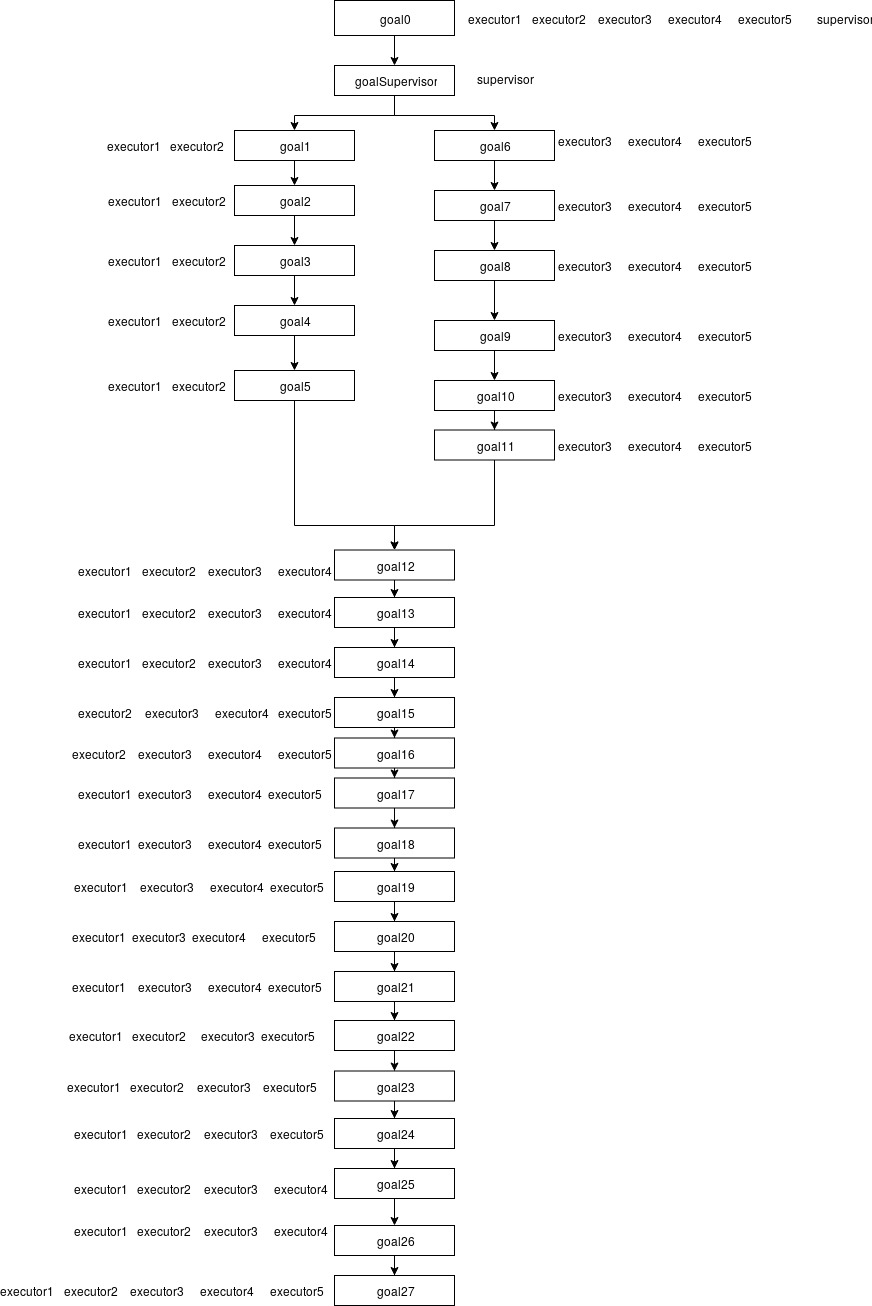
\includegraphics[width=1\linewidth]{diagramaDeObjetivos.jpg} 
  \caption{}
  \label{statediagram}
\end{figure}

\section{Raciocínios} 

Uma vez que o modelo foi definido e que foi implementado em um estudo de caso, é possível avaliar as conclusões possíveis dado certa condição de mundo. Essa seção demonstra como esse modelo cumpre o proposto por demonstrar certos raciocínios tendo em vista o caso de estudo em análise. 

\subsubsection{Raciocínio - 1} 


O raciocínio a seguir mostra o que acontece se o $agente4$ esquecer de passar o pano no bastão universal $relPanoGlicerina$ designados a ele no objetivo $goal1$. Todos os possíveis predicados vinculados a essa situação são;

\begin{enumerate}
	\item $hasRole(agente4,executor2)$ 
	\item $hasObligation(executor2,g1)$
	\item $hasRelation(g1,rg1)$ 
	\item $relPanoCorda \in rg1$
	\item $ x = agente4 $
	\item $tryReach(agente4,goal1)$
	\item $affects(relPanoGlicerina,relBastaoGarraCondutor)$
	\item $affects(relPanoGlicerina,relCordaEstropo)$  
	\item $affects(relPanoGlicerina,relChaveCatracaParafuso)$
	\item $affects(relPanoGlicerina,relParafusoConector)$ 
	\item $affects(relPanoGlicerina,relSoqueteParafuso)$ 
	\item $affects(relPanoGlicerina,relParafusoTorre)$
	\item $affects(relPanoGlicerina,relAgente4Corda)$ 
	\item $affects(relPanoGlicerina,relEstropoCorda)$	
\end{enumerate}

Com base nisso, as relações de implicabilidade resultantes são;

\begin{eqnarray}\nonumber
	hasRelation(goal1,rg1)\wedge \neg isPresent(relPanoGlicerina)  \nonumber \\ 
	\wedge (relPanoGlicerina\in rg_1) \wedge tryReach(agente4,goal1) \nonumber \\ 
	\to \nonumber \\ 
	violationRelation(agente4,g1,relPanoGlicerina) \nonumber \\	
\end{eqnarray}

\begin{eqnarray}\nonumber
	violationRelation(agente4,g1,relPanoGlicerina)  \nonumber \\ 
	\wedge affects(relPanoGlicerina,relBastaoGarraCondutor)   \nonumber \\ 
	\wedge hasPossibility(relBastaoGarraCondutor,false) \nonumber \\  
	\to \nonumber \\  
	hasPossibility(relBastaoGarraCondutor,true) 
\end{eqnarray}

\begin{eqnarray}\nonumber
	violationRelation(agente4,g1,relPanoGlicerina)  \nonumber \\ 
	\nonumber \\ 
	\wedge affects(relPanoGlicerina,relCordaEstropo)   \nonumber \\ 
	\wedge hasPossibility(relCordaEstropo,false) \nonumber \\  
	\to \nonumber \\  
	hasPossibility(relCordaEstropo,true) 
\end{eqnarray}

\begin{eqnarray}\nonumber
	violationRelation(agente4,g1,relPanoGlicerina)  \nonumber \\ 
	\nonumber \\ 
	\wedge affects(relPanoGlicerina,relParafusoConector)   \nonumber \\ 
	\wedge hasPossibility(relParafusoConector,false) \nonumber \\  
	\to \nonumber \\  
	hasPossibility(relParafusoConector,true) 
\end{eqnarray}

\begin{eqnarray}\nonumber
	violationRelation(agente4,g1,relPanoGlicerina)  \nonumber \\ 
	\nonumber \\ 
	\wedge affects(relPanoGlicerina,relSoqueteParafuso)   \nonumber \\ 
	\wedge hasPossibility(relSoqueteParafuso,false) \nonumber \\  
	\to \nonumber \\  
	hasPossibility(relSoqueteParafuso,true) 
\end{eqnarray}

\begin{eqnarray}\nonumber
	violationRelation(agente4,g1,relPanoGlicerina)  \nonumber \\ 
	\nonumber \\ 
	\wedge affects(relPanoGlicerina,relParafusoTorre)   \nonumber \\ 
	\wedge hasPossibility(relParafusoTorre,false) \nonumber \\  
	\to \nonumber \\  
	hasPossibility(relParafusoTorre,true) 
\end{eqnarray}

\begin{eqnarray}\nonumber
	violationRelation(agente4,g1,relPanoGlicerina)  \nonumber \\ 
	\nonumber \\ 
	\wedge affects(relPanoGlicerina,relAgente4Corda)   \nonumber \\ 
	\wedge hasPossibility(relAgente4Corda,false) \nonumber \\  
	\to \nonumber \\  
	hasPossibility(relAgente4Corda,true) 
\end{eqnarray}

\begin{eqnarray}\nonumber
	violationRelation(agente4,g1,relPanoGlicerina)  \nonumber \\ 
	\nonumber \\ 
	\wedge affects(relPanoGlicerina,relEstropoCorda)   \nonumber \\ 
	\wedge hasPossibility(rrelPanoGlicerinaelEstropoCorda,false) \nonumber \\  
	\to \nonumber \\  
	hasPossibility(relEstropoCorda,true) 
\end{eqnarray}

\begin{eqnarray}\nonumber
	violationRelation(agente4,g1,relPanoGlicerina)  \nonumber \\ 
	\nonumber \\ 
	\wedge affects(relPanoGlicerina,relEstropoCorda)   \nonumber \\ 
	\wedge hasPossibility(relEstropoCorda,false) \nonumber \\  
	\to \nonumber \\  
	hasPossibility(relEstropoCorda,true) 
\end{eqnarray}



\subsubsection{Raciocínio - 2} 

O raciocínio a seguir mostra o que acontece se o pano não estiver presente no local da manutenção quando os eletricistas forem alcançar o $goal1$. A lista a seguir exibe todos os predicados necessários para averiguar essa condição de mundo. 


\begin{enumerate}
	\item $hasRole(agente2,executor1)$ 
	\item $hasRole(agente3,executor1)$	 	
	\item $hasRole(agente4,executor2)$	 
	\item $hasObligation(executor1,g1)$
	\item $hasObligation(executor2,g1)$
	\item $tryReach(agente2,goal1)$ 
	\item $tryReach(agente3,goal1)$	 	
	\item $tryReach(agente4,goal1)$	
	\item $hasEntity(g1,eg1)$		
	\item $pano \in eg1$
	\item $\neg isPresent(pano)$
\end{enumerate}

\begin{eqnarray}\nonumber
	hasEntity(g1,eg1) \nonumber \\ 
	\wedge \neg isPresent(pano) 	\nonumber \\ 
	\wedge (pano \in eg1) \wedge tryReach(agente2,g1) \to \nonumber \\ 
	violationEntity(agent2,g1,pano) \nonumber \\
\end{eqnarray}

\begin{eqnarray}\nonumber
	hasEntity(g1,eg1) \nonumber \\ 
	\wedge \neg isPresent(pano) 	\nonumber \\ 
	\wedge (pano \in eg1) \wedge tryReach(agente3,g1) \to \nonumber \\ 
	violationEntity(agente3,g1,pano) \nonumber \\
\end{eqnarray}

\begin{eqnarray}\nonumber
	hasEntity(goal1,eg1) \nonumber \\ 
	\wedge \neg isPresent(pano) 	\nonumber \\ 
	\wedge (pano \in eg1) \wedge tryReach(agente4,g1) \to \nonumber \\ 
	violationEntity(agente4,g1,pano) \nonumber \\
\end{eqnarray}

\begin{eqnarray}
	violationEntity(agente4,goal1,pano) \to stopIn(goal1)
\end{eqnarray}



\subsubsection{Raciocínio - 3} 

O raciocínio a seguir mostra o que acontece se o $agente5$ tentar alcançar o objetivo $goal11$ com a umidade relativa do ar superior a setenta porcento. A lista a seguir exibe todos os predicados necessários para averiguar essa condição de mundo. 

\begin{enumerate}
	\item $hasRole(agente5,executor3)$
	\item $hasObligation(executor3,goal11)$	
	\item $tryReach(agente5,goal11)$ 
	\item $hasCondition(g11,cg1)$
	\item $umidade70 \in cg1$	
	\item $\neg isPresent(umidade70)$
	\item $hasRisk(umidade70,eletrocutado,morte)$
\end{enumerate}

\begin{eqnarray}
	hasCondition(goal11,cg1) \nonumber \\ 
	\wedge \neg isPresent(umidade70) \nonumber \\
	\wedge umidade70 \in cg1 \nonumber \\
	\wedge tryReach(agente5,g11) \to \nonumber \\  
	violationCondition(agente5,g11,umidade70) \nonumber \\
\end{eqnarray}

\begin{eqnarray} \nonumber
	violationCondition(agente5,goal11,umidade70) \nonumber \\
	\wedge hasRisk(umidade70,eletrocutado,morte) \to \nonumber \\  
	consequenceOfBadEvent(g11,agente5,eletrocutado,morte)
\end{eqnarray}


\begin{eqnarray}
	consequenceOfBadEvent(g11,agente5,eletrocutado,morte) \to stopIn(g11)
\end{eqnarray}
\subsubsection{Raciocínio - 4} 

O raciocínio a seguir mostra o que acontece se o $agente3$ errar a forma adequada de realizar o relacionamento $relChaveCatracaParafuso$ no objetivo $goal15$. Os predicados envolvidos são;

\begin{enumerate}
	\item $hasRole(agente4,executor2)$
	\item $hasObligation(executor4,goal15)$	
	\item $tryReach(agente4,g15)$ 
	\item $hasRelation(g15,rg15)$
	\item $relChaveCatracaParafuso \in rg15$	
	\item $\neg isPresent(relChaveCatracaParafuso)$
	\item $hasRisk(relChaveCatracaParafuso,eletrocutado,morte)$
\end{enumerate}

\begin{eqnarray}
	hasRelation(goal15,rg15) \nonumber \\
	\wedge \neg isPresent(relChaveCatracaParafuso)  \nonumber \\ 
	\wedge (relChaveCatracaParafuso \in rg15) \nonumber \\
	\wedge tryReach(agente4,g15) \nonumber \\ 
	\to \nonumber \\ 
	violationRelation(agente4,g15,relChaveCatracaParafuso) \nonumber \\
\end{eqnarray}

\begin{eqnarray}\nonumber
	violationRelation(agente4,g15,relChaveCatracaParafuso) \nonumber \\ 
	 \wedge hasRisk(relChaveCatracaParafuso,eletrocutado,morte) \nonumber \\ 
	\to \nonumber \\ 
	consequenceOfBadEvent(g15,agente4,eletrocutado,morte)
\end{eqnarray}

\begin{eqnarray}
	consequenceOfBadEvent(g15,agente4,eletrocutado,morte) \to stopIn(g15)
\end{eqnarray}

\subsubsection{Raciocínio - 5} 

A finalidade dessa demonstração consiste em mostrar como um agente pode ser submetido a consequências ruins tendo em vista erros cometidos por outros profissionais. O raciocínio 1 mostra que o fato do $agente4$ não conseguir realizar o relacionamento $relPanoGlicerina$ resulta na violação $violationRelation(agente4,goal1,relPanoGlicerina)$. Essa violação, por sua vez, impacta diversas outras relações, em que $hasPossibility(relParafusoTorre,true)$ é uma delas. Assim sendo, antes do $agente4$ cometer o erro, a possibilidade da ocorrência de um evento ruim acontecer era 0, se o agente realizar a relação $relParafusoTorre$ sem cometer violação alguma. Contudo, após a ocorrência do erro cometido pelo $agent4$, existe uma possibilidade de um evento ruim acontecer na relação $relParafusoTorre$ mesmo que tudo seja feito de acordo com os conformes. Assim sendo, a lista de predicados e o raciocínio mostra o que acontece dado a seguinte situação; o possível evento ruim presente em $relParafusoTorre$ se torna uma realidade;  

\begin{enumerate}
	\item $relParafusoTorre \in rg19$	
	\item $hasRelation(g19,rg19)$		
	\item $hasObligation(executor3,g19)$
	\item $hasObligation(executor4,g19)$
	\item $hasObligation(executor5,g19)$		
	\item $tryReach(agente5,g19)$
	\item $tryReach(agente6,g19)$
	\item $tryReach(agente7,g19)$									
	\item $hasRole(agente5,executor3)$
	\item $hasRole(agente6,executor4)$
	\item $hasRole(agente7,executor5)$
	\item $hasRisk(relParafusoTorre,eletrocutado,morte)$
	\item $hasPossibility(relParafusoTorre,true)$
	\item $happensBadEvent(g19,relParafusoTorre)$	
\end{enumerate}


\begin{eqnarray}\nonumber
	hasRelation(g19,rg19) \nonumber
	\wedge (relParafusoTorre \in rg19) \nonumber \\ 
	happensBadEvent(g19,relParafusoTorre)  \nonumber \\
	\wedge hasRisk(relParafusoTorre,eletrocutado,morte) \nonumber \\ 
	\wedge tryReach(agente5,g19) \nonumber \\ 
	\to \nonumber \\ 
	consequenceOfBadEvent(goal19,agente5,eletrocutado,morte)
\end{eqnarray}

\begin{eqnarray}
	consequenceOfBadEvent(g19,agente5,eletrocutado,morte) \to stopIn(g19)
\end{eqnarray}

\begin{eqnarray}\nonumber
	hasRelation(g19,rg19) \nonumber
	\wedge (relParafusoTorre \in rg19) \nonumber \\ 
	\wedge happensBadEvent(g19,relParafusoTorre)  \nonumber \\
	\wedge hasRisk(relParafusoTorre,eletrocutado,morte) \nonumber \\ 
	\wedge tryReach(agente6,g19) \nonumber \\ 
	\to \nonumber \\ 
	consequenceOfBadEvent(goal19,agente6,eletrocutado,morte)
\end{eqnarray}

\begin{eqnarray}
	consequenceOfBadEvent(g19,agente6,eletrocutado,morte) \to stopIn(g19)
\end{eqnarray}

\begin{eqnarray}\nonumber
	hasRelation(g19,rg19) \nonumber
	\wedge (relParafusoTorre \in rg19) \nonumber \\ 
	\wedge happensBadEvent(g19,relParafusoTorre)  \nonumber \\
	\wedge hasRisk(relParafusoTorre,eletrocutado,morte) \nonumber \\ 
	\wedge tryReach(agente7,g19) \nonumber \\ 
	\to \nonumber \\ 
	consequenceOfBadEvent(goal19,agente7,eletrocutado,morte)
\end{eqnarray}

\begin{eqnarray}
	consequenceOfBadEvent(g19,agente7,eletrocutado,morte) \to stopIn(g19)
\end{eqnarray}


\subsubsection{Raciocínio - 6}

O objetivo $g23$ deve ser atingido pelos agentes com as funções de $executor1$,$executor2$,$executor3$ e $executor5$. Isso implica dizer que os agentes; $agente2$,$agente3$,$agente4$,$agente5$ e $agente7$ devem tentar alcançar esses resultados. Considerando que $agg23$ são todos os agentes que tentaram alcançar o objetivo e $ago23$ os agentes que são obrigados a fazer isso, segue o raciocínio;


\begin{enumerate}
	\item $agente2 \in agg23$	
	\item $agente3 \in agg23$
	\item $agente4 \in agg23$
	\item $agente5 \in agg23$
	\item $agente7 \in agg23$								
	\item $agente2 \in ago23$	
	\item $agente3 \in ago23$
	\item $agente4 \in ago23$
	\item $agente5 \in ago23$
	\item $agente7 \in ago23$	
	\item $ago23 \subset agg23$
	\item $\neg stopIn(g23,agg23)$										
\end{enumerate}

\begin{eqnarray}\label{rel15}
	\neg stopIn(g23,agg23) \wedge (agg23 \subset ago23) \to isReached(g23)
\end{eqnarray}

\subsubsection{Raciocínio - 7}

O raciocínio para o caso onde $agente1$ tente alcançar o objetivo $g23$.  

\begin{enumerate}
	\item $hasRole(agente1,supervisor)$
	\item $hasObligation(agente1,g23) \to F$										
\end{enumerate}

Isso implica em uma afirmação falsa, então esse mundo não é possível segundo o modelo implementado para este estudo de caso.

\subsection{Trabalhos Correlatos}

Essa seção tem como finalidade realizar uma análise comparativa do modelo proposto neste estudo com os modelos atuais sobre sistemas multiagentes normativos. Cada uma das próximas seções aborda um modelo diferente.

\subsubsection{MOISE+}

O Moise+ é usado para realizar a especificação de sistemas multiagentes. Para cumprir com essa finalidade, existe três tipos de especificação que são; Estrutural, Funcional, e Deôntica. 

A especificação estrutural acontece em três níveis, individual, social e coletivo. O nível individual trata de definir os papeis $\rho$ dos agentes. Uma possível entre os papeis acontece por intermédio da hereditariedade em que se $\rho'$ é filho de $\rho$. Isso implica afirmar que $\rho'$ é uma especialização de $\rho$. Um exemplo apropriado para isso é o jogo de futebol onde existe o papel jogador dado por $\rho$ e existe o papel atacante dado por $\rho'$ \cite{mosieframework}. Em termos formais, essa relação é dada pro; 
\begin{eqnarray}\nonumber
\rho_a \sqsubset \rho_b
\end{eqnarray}

O nível social estabelece relações de ligação dado pelo predicado $link(\rho_s,\rho_d,t)$. Existe três possíveis valores para $t$, os quais são $t = \{aut, com, acq\}$. O valor $auth$ significa autoridade (neste caso $\rho_s$ exerce autoridade sobre $\rho_d$), o valor $com$ significa comunicação (neste caso $\rho_s$ pode se comunicar com $\rho_d$) e o valor $acq$ significa conhecimento ($\rho_s$ tem conhecimento da existência de $\rho_d$) \cite{mosieframework}. O MOISE+ define as seguintes relações de implicabilidade

\begin{eqnarray}\nonumber
	link(\rho_s,\rho_d,auth) \to link(\rho_s,\rho_d,com) \nonumber \\
	link(\rho_s,\rho_d,com) \to link(\rho_s,\rho_d,acq) 
\end{eqnarray}

O modelo também determina como se dá as relações de hereditariedade para o predicado de $link$, é dado por \cite{mosieframework}; 

\begin{eqnarray}\nonumber
	link(\rho_s,\rho_d,t) \wedge \rho_s' \sqsubset \rho_s' \to link(\rho_s',\rho_d,t) \nonumber \\
	link(\rho_s,\rho_d,t) \wedge \rho_d' \sqsubset \rho_d' \to link(\rho_s,\rho_d',t) 	
\end{eqnarray}


O nível coletivo determina a existência de compatibilidade entre os papeis \cite{mosieframework}. Essa é uma relação reflexiva e transitiva de determina que se um papel $\rho_a$ possui a capacidade de realizar um determinado objetivo, então o papel $\rho_b$ também tem essa capacidade. Em termos formais, essa relação se dá da seguinte forma \cite{mosieframework}.;

\begin{eqnarray}\nonumber
	\rho_a \bowtie \rho_b \wedge \rho_a \neq \rho_b \wedge \rho_a \sqsubset \rho' \to \rho' \bowtie \rho_b 
\end{eqnarray}

O nível coletivo também apresenta o conceito de grupo dado por $gt$ e constituído por;

\begin{eqnarray}\nonumber
	gt = \langle R,SG,L^{intra},L^{inter},C^{intra},C^{inter},np,ng\rangle 
\end{eqnarray}

Em que $R$ é o conjunto dos papeis não abstratos, $SG$ são subgrupos que estão contidos neste grupo, $L^{intra}$ consiste dos $links$ intra-grupos, $L^{inter}$ dos links inter-grupos, $C^{intra}$ das relações de compatibilidade intra-grupos e $C^{inter}$ das relações de compatibilidade inter-grupos. O símbolo $np$ denota a cardinalidade mínima e máxima para uma dada função e o símbolo $ng$ realiza o mesmo para os subgrupos \cite{mosieframework}. 

A Especificação Funcional tem como por finalidade descrever os objetivos a serem atingidos dentro de uma estrutura de árvore. A figura a seguir define como se dá esse tipo de especificação; 

\begin{figure}[H]
  \centering
  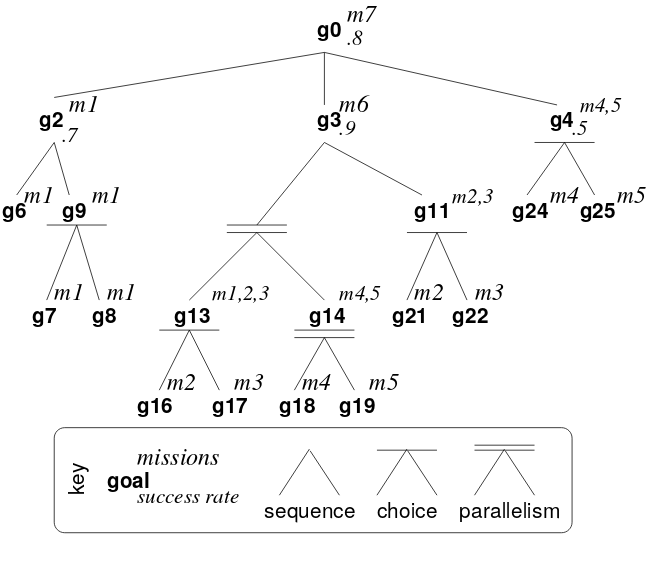
\includegraphics[width=0.8\linewidth]{figmoise} 
  \caption{Arvore de objetivos definido pelo modelo Moise \cite{mosieframework}}
  \label{arvoremoise}
\end{figure}

A figura \ref{arvoremoise} define três tipos de relação de subobjetivos; $sequence$ onde todos os subobjetivos devem necessariamente ser concluídos em sequência, $choice$ onde o agente tem a possibilidade de escolher qual objetivo ele deseja seguir e $parallelism$ onde todos os objetivos devem ser concluídos, contudo sem uma sequência definida. Como é possível observar na figura, os objetivos são agrupados em conjuntos de missões $m$. A relação a seguir define isso melhor;

\begin{eqnarray}\nonumber
	m_k = \{ g_n,...,g_m\}
\end{eqnarray}


A Especificação Deôntica define predicados para estabelecer permissões e obrigações entre os papeis e as missões. Toda obrigação implica necessariamente em uma permissão. A relação a seguir estabelece isso; 

\begin{eqnarray}\nonumber
	obl(\rho,m,tc) \to per(\rho,m,tc) \\
	obl(\rho,m,tc) \wedge \rho \sqsubset \rho' \to obl(\rho',m,tc) \\
	per(\rho,m,tc) \wedge \rho \sqsubset \rho' \to per(\rho',m,tc) \\	
\end{eqnarray}

Onde o predicado $obl$ define uma obrigação e o predicado $per$ define permissão. O argumento $tc$ define uma periodicidade de tempo para o qual a relação deôntica é valida. 

Existe muitos ponto similares entre o modelo proposto neste estudo e o Moise. Ambos os modelos apresentam papeis $\rho$, apresentam objetivos $g$ e apresentam relações deônticas de obrigação e permissão. Isso se deve ao fato, em partes, que o modelo proposto neste estudo importou muitos dos conceitos presentes no Moise tendo em vista a aplicabilidade para o domínio em interesse. Esses conceitos são importantes para o modelo deste estudo pois são grande relevância para descrever situações onde uma equipe de pessoas devem atingir certos objetivos trabalhando em cooperação. 

Contudo, ambos modelos apresentam diferenças significativas. Uma dessas diferenças reside em como as relações deônticas são atribuídas, pois no Moise a relação é feita entre o papel e a missão e no modelo proposto neste estudo a relação é feita entre o papel e o objetivo. Isso se deve ao fato de que uma das finalidades deste estudo consiste na realização de uma análise de sanções e violações. Como essas analises trabalham no nível de atividades, objetos e condições (dentro do contexto deste estudo), trabalhar na ordem de objetivos trás uma análise mais aprimorada no estudo das violações e sanções. 

O Moise não apresenta suporte a tratativa de sanções e violações. Assim sendo, para conseguir atingir um modelo onde fosse possível analisar certos tipos de sanções e violações de interesse, foi necessário introduzir predicados que não fazem parte do vocabulário e da sintaxe do Moise. 

O Moise trabalha uma estrutura lógica de interesse a descrição de grupos, \textit{links} e compatibilidades. Esses conceitos não são trabalhados no modelo em interesse por não serem necessários ao domínio de interesse deste estudo. Assim sendo, esses conceitos trariam complexidades adicionais sem justificativa válida para isso.


\subsection{\textit{Normative Multi-Agent Programs and Their Logics}}

O texto \cite{dastaniNormativeMultiAgentProgram} apresenta um modelo com a finalidade de descrever agentes normativos com a capacidade de cometer uma certa violação. O modelo define sanções para as violações. O estudo estrutura o modelo como uma linguagem de programação (usando a notação EBNF) onde os problemas de sistemas multiagentes são tratados como programas escritos neste linguagem \cite{dastaniNormativeMultiAgentProgram}. Assim sendo, um programa de sistemas multi-agentes é descrito como sendo; 


\begin{figure}[H]
  \centering
  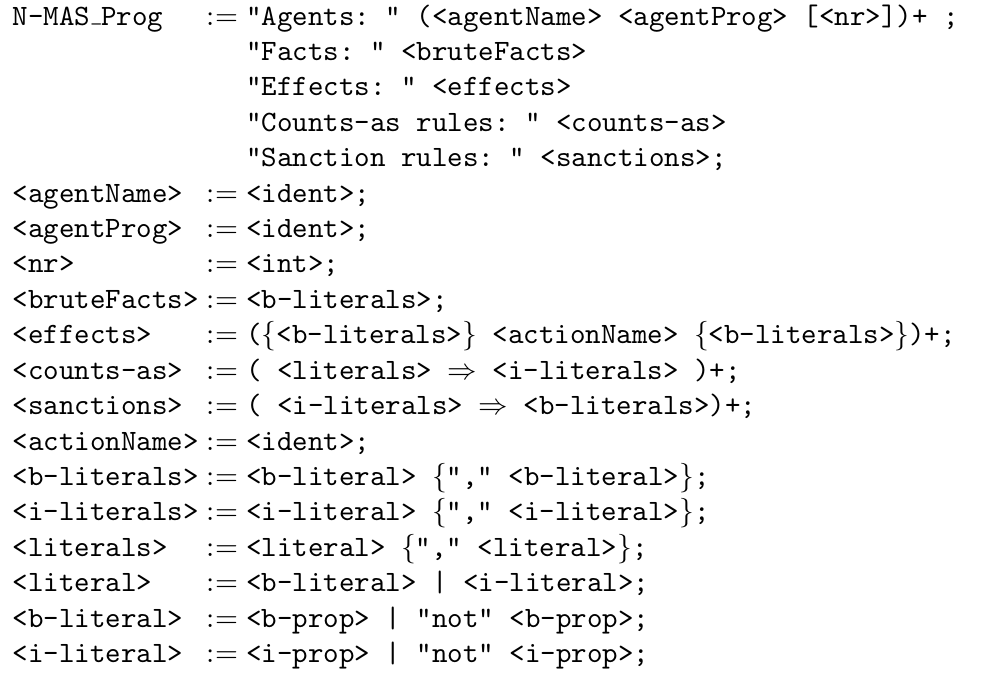
\includegraphics[width=0.8\linewidth]{masprogram.png} 
  \caption{Linguagem para descrever um programa de multiagentes normativos com a possibilidade de violações e sanções na notação EBNF segundo o texto \cite{dastaniNormativeMultiAgentProgram}. Nesta notação, $<ident>$ é usado para denotar uma \textit{string} e $<int>$ inteiros. Os termos $<b-prop>$ e $<i-prop>$ são usados para designar dois tipos de conjuntos de proposições que são disjuntos entre sí}
  \label{descreveprograma}
\end{figure}

Com base no proposto por esse modelo, um programa de sistemas multiagentes é descrito por \textit{Agents} (agentes), \textit{Facts} (fatos), \textit{Effects} (efeitos), \textit(Count-as rules) (regras que determinam o adequado comportamento do agente), \textit{Sanction rules} (regras de sanção) \cite{dastaniNormativeMultiAgentProgram}. 

Os \textit{Agents} são definidos em termos de duas \textit{strings} e um inteiro. A primeira \textit{string} é \textit{agentName} e é usado para definir o nome do agente e a segunda \textit{string} é \textit{agentProg} e define o nome  do arquivo onde se encontra especificações do respectivo agente. O inteiro \textit{nr} é usado para definir a quantia do agente \cite{dastaniNormativeMultiAgentProgram}.

Os \textit{Facts} são compostos por conjuntos de literais denominados de \textit{bruteFacts}. Esses são fatos onde ocorre uma violação que desencadeia em uma dada sanção \cite{dastaniNormativeMultiAgentProgram}. 

Os \textit{Effects} são compostos por \textit{effects}. Estes, por sua vez, são estruturados em termos de \textit{b-literals} (conjuntos que contem literais onde estes, por sua vez, representam um dado estado de mundo), e \textit{actionName} onde este, por sua vez, descreve ações que geram trasições de um estado de mundo para outro estado \cite{dastaniNormativeMultiAgentProgram}. 

Os \textit{Count-as rules} são compostos por \textit{counts-as}. Esses, por sua vez, definem regras normativas. Isso implica em relações de implicabilidade que resultam em uma dada violação \cite{dastaniNormativeMultiAgentProgram}. 

Os \textit{Sanction rules} são estruturados por \textit{sanctions}. Esses, por sua vez, definem regras de implicabilidade que competem a uma tratativa da violação \cite{dastaniNormativeMultiAgentProgram}.
 
A figura a seguir ilustra um exemplo de um programa de sistema multiagente escrito nesta linguagem;


\begin{figure}[H]
  \centering
  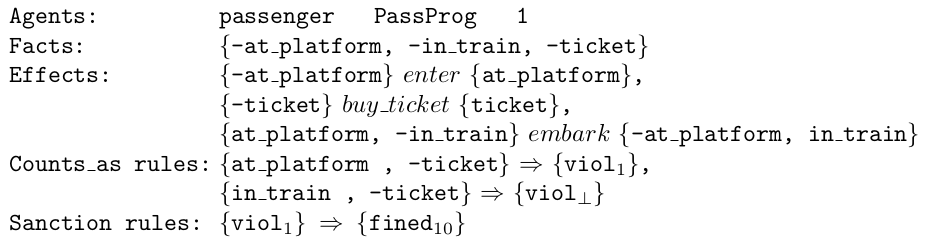
\includegraphics[width=0.8\linewidth]{programdastani.png} 
  \caption{Um programa descrito na linguagem proposta neste estudo onde um agente representa um passageiro em uma estação de trem que pode entrar com ou sem um \textit{ticket} na plataforma e no trem \cite{dastaniNormativeMultiAgentProgram}.}
  \label{exemploprograma}
\end{figure}


A figura \ref{exemploprograma} apresenta um programa que contem um agente com nome \textit{passenger}. O agente pode estar ou não na plataforma e no trem, sem ou com \textit{ticket}. Se o agente entrar na plataforma ou no trem sem o \textit{ticket}, então esse agente cometeu uma violação. Para este programa, a sanção da violação que ocorre por entrar na plataforma sem o \textit{ticket} resulta em uma punição onde o agente deve pagar 10 Euros pelo ocorrido \cite{dastaniNormativeMultiAgentProgram}.

O modelo presente em \cite{dastaniNormativeMultiAgentProgram} apresenta muitas similaridades ao modelo definido neste estudo sobre o ponto de vista de sanção e violação, uma vez que a raiz para os conceitos de ambos os estudos advêm das mesmas origens. Contudo, o modelo \cite{dastaniNormativeMultiAgentProgram} apresenta um aspecto muito mais abrangente podendo considerar uma vastidão de mundos possíveis. Isso pois esse modelo não define conceitos como (objetivos, artefatos, riscos, possibilidades). Já no modelo deste estudo, esses conceitos e predicados são definidos.

Portanto ambos os modelos podem ser usados para delimitar o estudo de caso presente neste texto, com a diferença que o modelo deste estudo apresenta uma linguagem que delimita com maior rigor o problema em análise do que o modelo \cite{dastaniNormativeMultiAgentProgram}.

\subsection{\textit{V3S: A Virtual Environment for Risk-Management Training Based on Human-Activity Models}}

V3S é um modelo com a finalidade de gerar ambientes para desenvolver treinamentos complexos em ambiente de realidade virtual visando atividades de risco e de emergência. O modelo é composto por três submodelos; \textit{Domain Model}, \textit{Activity Model} e \textit{Risk Model} \cite{violationcamille}. O \textit{Domain Model} é o núcleo do sistema. Todos os objetos, ações e relações são descritos por uma ontologia. A figura \ref{domainmodel} exibe a estrutura de classe desta ontologia.

\begin{figure}[H]
  \centering
  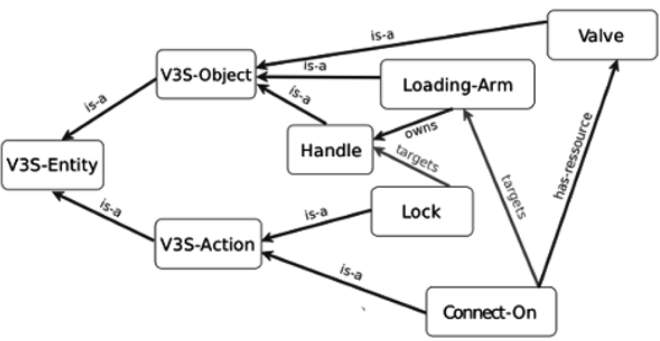
\includegraphics[width=0.5\linewidth]{ontologyv3.png} 
  \caption{Ontologia que descreve \textit{Domain Model} no model V3S \cite{violationcamille}}
  \label{domainmodel}
\end{figure}


\textit{Activity Model} é estruturado sobre uma linguagem de descrição conhecido por \textit{ACTIVITY-DL}. Essa linguagem usa álgebra de Allen's que tem como por finalidade definir raciocínios temporais \cite{Allen}. As relações definidas por essa álgebra é dada por; 
\begin{enumerate}
	\item $X < Y$ onde $X$: ocorre antes de $Y$ 
	\item $X m Y$,$Y mi X$: $X$ encontra $Y$
	\item $X o Y$, $X oi Y$: $X$ sobrepõem a $Y$
	\item $X s Y$, $Y si X$: $X$ começa $Y$
	\item $X d Y$, $Y di X$: $X$ ocorre durante $Y$	  
	\item $X f Y$, $Y fi X$: $X$ termina junto com $Y$	  	
	\item $X = Y$ $X$ é igual a $Y$	  		
\end{enumerate}

A linguagem define construtores que são semanticamente equivalente a certos operadores da álgebra de Allen's. Esses construtores (atuantes sobre atividades) são definidos pela tabela \ref{acticonstruct}

\begin{table}[H]
\centering
\begin{tabular}{|l|l|l|}
\hline
Construtor & Nome         & Relações de Allen \\ \hline
IND        & Independent  & $A\{<,>,m,mi,o,oi,s,si,d,di,f,fi,=\}B$\\ \hline
SEQ        & Sequential   & $A\{<,>,m,mi\}B$\\ \hline
SEQ-ORD    & Ordered      & $A\{<,>,m\}B$\\ \hline
PAR        & Parallel     & $A\{o,oi,s,si,d,di,f,fi,=\}B$ \\ \hline
PAR-SIM    & Simultaneous & $A\{=\}B$\\ \hline
PAR-START  & Start        & $A\{s,si,=\}B$\\ \hline
PAR-END    & End          & $A\{f,fi,=\}B$ \\ \hline
\end{tabular}
\caption{Construtores da linguagem \textit{ACTIVITY-DL} \cite{violationcamille}}
\label{acticonstruct}
\end{table}

No que tange a questões referentes a segurança e violação, a linguagem \textit{ACTIVITY-DL} define \textit{tags} no estudo \cite{FADIER2003759}. Essas \textit{tags} são BCTUs,BATUs. BCTUs representam situações informais entre os atores de um determinado campo, por exemplo; trabalhar com produtos químicos sem usar equipamentos de proteção individual. BATUs corresponde a práticas de risco tolerado. Existe dois tipos de BATUs, primeiro - quando realizado por obrigação ou interesse de conforto (quando os operadores acham impossível realizar a operação respeitando as instruções), segundo - ocorre durante a operação do sistema com o propósito de evitar que o sistema deixe de funcionar.    

\textit{Activity Model} apresenta uma categorização de pré-condições. A tabela \ref{precondition} detalhe essa categorização. 

\begin{table}[]
\begin{tabular}{|l|l|p{0.6\linewidth}|}
\hline
\textbf{Categoria} & \textbf{Pré-condição} & \textbf{Descrição}                                                                                                                                                                                                                                              \\ \hline
Condições para perceber  & Nomológico            & Descreve o estado do mundo necessário para que a tarefa seja fisicamente realizável. Condições dependem diretamente das regras de ação definidas no modelo de domínio. Exemplo: Abre a porta se estiver fechada.                                                \\ \hline
Condições para perceber  & Regulamentar          & Descreve o estudo do mundo necessário para uma boa realização da atividade de acordo com prescrito em procedimento. Exemplo: Para desconectar o tubo, a proteções devem ser desgastado.                                                                         \\ \hline
Condições para  Examinar & Contextual            & Descreve o estado de mundo em que a atividade é relevante. Quando essa condição é falsa, então a atividade deve ser ignorada. Exemplo: Limpar o tubo é relevante apenas se o tubo estiver sujo.                                                                 \\ \hline
Condições para  Examinar & Favorável             & Descreve o estado de mundo onde a tarefa é preferencial sobre as demais. Essas condições ajudam a escolher entre várias tarefas quando existe uma alternativa para a realização de uma tarefa decomposta. Exemplo: se o parafuso estiver enferrujado, desarmar. \\ \hline
\end{tabular}
\caption{As pré-condições possíveis para as atividades \cite{violationcamille}}
\label{precondition}
\end{table}

\textit{Risk Models} é a parte do modelo que define a análise de risco. Existe duas categorias; risco de análise clássico e método de análise de confiabilidade humana. A primeira categoria permite definir uma análise quantitativa de risco, contudo falha ao definir a complexidade dos resultados frente a fatores humanos. Em contrapartida, a segunda categoria considera fatores humanos, contudo falha em definir medidas o objetivas sobre questões de segurança \cite{violationcamille}.

O \textit{V3S} combina ambas situações usando a abordagem MELISSA \cite{Camus2012}\cite{violationcamille}. Essa abordagem é baseada em três pontos (1) atividades relacionadas em cenários de acidentes, (2) descrição das tarefas de representação e (3) fatores influentes em potencial nas atividades. 

O \textit{V3S} possue representações para defini as entidades, objetos e ações assim como o modelo proposto neste estudo. Contudo, existe diferenças na estrutura ontológica de ambo os modelos, pois o \textit{V3S} define tanto objetos e ações como entidades, enquanto que o modelo proposto neste estudo apenas objetos são entidades. O \textit{V3S} não caracteriza os agentes dentro de sua estrutura ontológica, enquanto que o modelo deste estudo faz isso definindo os agentes como entidades que se relacionam com outras entidades. 

No que tange a questões referentes as atividades, o \textit{V3S} realiza a descrição sequencial das mesmas por intermédio da álgebra de \textit{Allen's}, enquanto que este estudo usa uma abordagem mais simples para representar as relações entre objetivos usando apenas alguns predicados para tratar essa dinâmica. O mesmo ocorre para as pré-condições, onde o \textit{V3S} detalha os tipos de pré-condições existentes enquanto que o modelo presente neste estudo não faz isso.

O \textit{V3S} realiza a tratativa de violações usando o estudo \cite{FADIER2003759}. Em contraste com isso, neste modelo os pesquisadores optaram por definir as violações por intermédio de regras (definidas por meio de relações de implicabilidade) onde define claramente quais condições resultam numa determinada violação. Com base nisso, a proposta do modelo deste texto está muito mais próximo do texto \cite{dastaniNormativeMultiAgentProgram} do que do \textit{V3S}. 

O \textit{V3S} não exerce uma definição objetiva e formal das sanções. O modelo proposto neste texto também não apresenta classes ou predicados que tornam explícito as relações de sanção. Contudo, esse estudo usa a abordagem acadêmica clássica (usada também no estudo \cite{dastaniNormativeMultiAgentProgram}) tratando as sanções como consequências de uma violação. O \textit{V3S} aprenta esse tipo de situação, contudo sem o formalismo de sanção. 

O modelo proposto neste estudo define as violações em três categorias (condição, relações e entidades), algo que o \textit{V3S} não aborda. Isso não significa afirmar que o \textit{V3S} não pode ser usado para modelar essas violações, contudo, este modelo possui um vocabulário para resolver os problemas deste tipo de violação de forma muito mais específica quando comparado ao \textit{V3S}. 

Os riscos também são tratados diferentemente em ambos os estudos. O \textit{V3S} usa uma abordagem robusta baseada em estudos acadêmicos envolvendo segurança. O modelo deste estudo trata essa questão de forma mais simples, específica e objetiva. Isso, pois, risco é tratado com base na \textit{NR.1.7} sobre a perspectiva de mapa de riscos. 

\subsubsection{NormMAS}

\textit{NormMAS} é um modelo usado para definir comportamento normativo de sistemas multiagentes \cite{chang}. No que tange questões referentes ao comportamento normativo, o modelo trabalha com duas definições \cite{chang}. A primeira definição é;

\textbf{Definição 1.} \textit{Um norma é definida por meio de uma tupla} $N = \langle \mu,\kappa,\chi,\tau,\rho \rangle$

\begin{itemize}
    \item $\mu \in \{obligation,prohibition\}$ representa as modalidades de norma.
    \item $\kappa \in \{action,state\}$ representa o tipo de \textit{trigger} da condição.
    \item $\chi$ representa o conjunto de estados em que uma norma se aplica.
    \item $\tau$ representa a norma da condição de \textit{trigger}
    \item $\rho$ representa a sanção aplicava pela violação do agente.
\end{itemize}

A defição 1 pode ser compreendida sobre o seguinte exemplo; 

\textit{Todos os imigrantes que possuem passaporte válido, devem ser aceitos. A falha resulta na perda de 5 créditos}. 

Dentro da definição 1, o exemplo fica;

\begin{eqnarray}
    \langle obligation,action,valid(Passport),accept(Passport),loss(5)\rangle
\end{eqnarray}

\textit{NormMAS} define um \textit{Registro de ação} que é dado pela definição 2. 

\textbf{Definição 2.} \textit{Um Registro de Ação é definido por meio de uma tupla} $R = \langle \gamma,\alpha,\beta \rangle$

\begin{itemize}
    \item $\gamma$ representa o agente executando uma ação;
    \item $\alpha$ representa a ação sendo executada pelo agente $\gamma$
    \item $\beta$ representa os estados internos do agente $\gamma$ no momento da execução.
\end{itemize}

Assim como o modelo definido neste estudo, \textit{NorMAS} formaliza o conceito de norma em conjunto com o conceito de violação e de sanção. Contudo, assim como o estudo \cite{dastaniNormativeMultiAgentProgram}, \textit{NormMAS} pode ser usado para representar o caso em estudo, contudo o engenheiro de modelagem teria de elaborar diversos conceitos - como riscos, fatalidades, condições a serem mantidas durante a execução da atividade, definir como um objetivo afeta outro e relacionamentos. Em contraste com isso, o modelo presente neste estudo não apresenta a abrangência que o \textit{NormMAS} apresenta, contudo delimita com maior rigor o vocabulário a ser usado pelo engenheiro de modelagem.

\bibliographystyle{sbc}
\bibliography{sbc-template}
\end{document} 
	
